\chapter{コメントアウトした}



\section{再生性}
\subsubsection{$(\star)$ $N(\mu,\sigma^2)$に従う確率変数であることを判定できるか}
$N(0,1)$に従う確率$x_1,x_2,\cdots,x_n$から計算した統計量、$z=\frac{\bar{X}-0}{\sqrt{\frac{1}{n}}}$は、$N(0,1)$に従い、$z$が$95\%$の確率で見つかる範囲は$[-1.96,1.96]$である。
同様に、$y_1,y_2,\cdots,y_n \sim N(1.96,1)$であるならば、$z=\frac{\bar{Y}-1.96}{\sqrt{\frac{1}{n}}}$は、$N(0,1)$に従う。

確率変数から、特定の母数を持つ正規分布に従わないことを示すことはできるだろうか。
具体的な問題設定として、
$y_1,y_2,\cdots,y_n$を正規分布に従う確率変数とする。そのとき、$y_1,y_2,\cdots,y_n$が$N(\mu,\sigma^2)$に従わないことを判断する良い方法はどのようなものだろうか。

ここで、$y_1,y_2,\cdots,y_m \sim N(1.96,1)$にもかかわらず、$N(0,1)$に従うと推測した場合、$z=\frac{\bar{Y}-0}{\frac{1}{\sqrt{n}}} \sim N(0,1)$であると考えられる。
$z$の分子の$\mu$が$0$になっていることに注意が必要である。
実際に、$y_1,y_2,\cdots y_{100}$を$N(1.96,1)$からサンプリングした標本を$100$個作ってみると、およそ$19$を中心に分布することがわかる。
このことは、$y_1,y_2,\cdots,y_m\sim N(0,1)$であるならば、$z$は、$[-1.96,1.96]$の間で$95\%$の確率で入るので、この推測が間違いであることが推測される。
以上の考察から、$y_1,y_2\cdots,y_n\sim N(0,1)$ではないと判断する。

\begin{figure}
    \begin{center}
        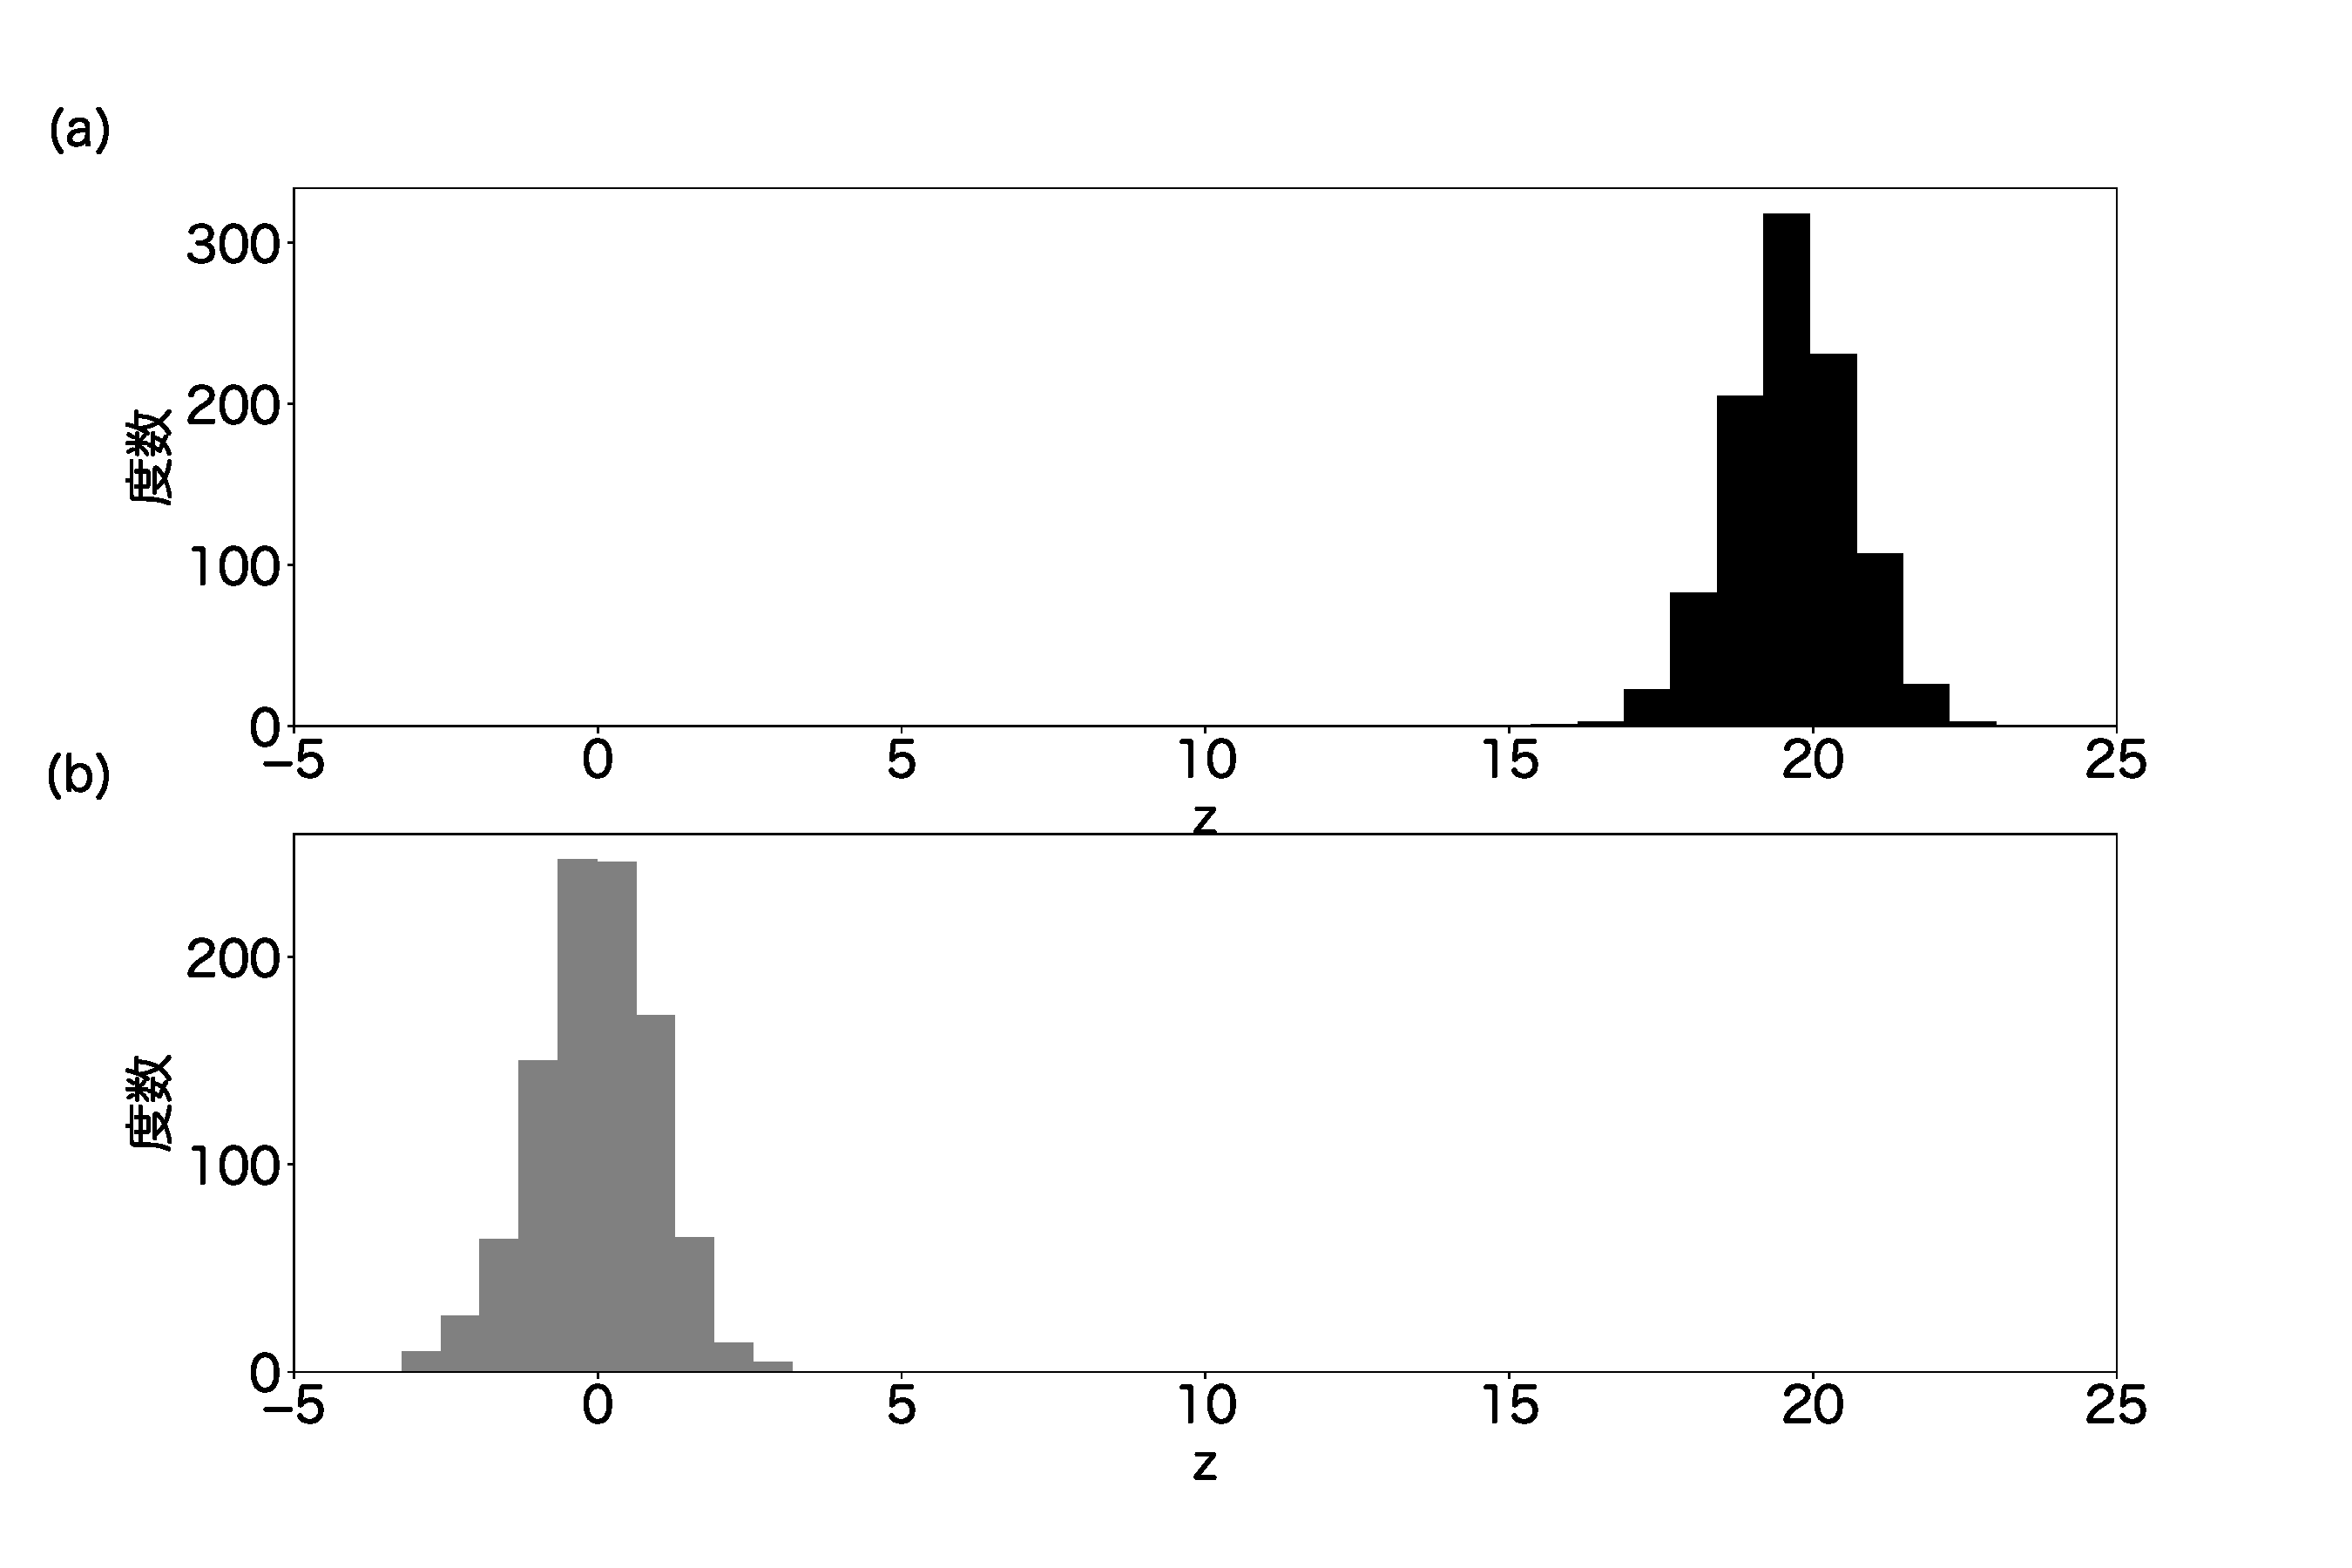
\includegraphics[width=15cm]{./image/02_/normal_distribution_test.pdf}
        \caption{(a)$N(1.96)$に従う確率変数を100個サンプリングし、その標本を1000個集めたときの$z=\sqrt{100}(\bar{X}-0)$のヒストグラム (b)$N(0,1)$に従う確率変数を100個サンプリングし、その標本を1000個集めたときの$z=\sqrt{100}(\bar{X}-0)$値のヒストグラム}
    \end{center}
\end{figure}


もう一つ例を挙げる。
$y_1,y_2,\cdots,y_n \sim N(170,5.8)$とする。このとき、この標本が$N(168,5.8)$によりサンプリングされたものではなくことを示すことはできるだろうか。
$z=\sqrt{n}\frac{\bar{y}-168}{\sigma}$を計算すればよい。
図には、$N(170,5.8)$に従う確率変数を100個サンプリングし、その標本を1000個集め、ヒストグラムを描いた。
これをみると、$0.5$を中心に分布が広がることがわかる。$z=\frac{\bar{X}-168}{\sqrt{\frac{5.8}{n}}}\sim N(0,1)$であるはずである。
複数回、標本を得た場合でも、$z$が$[-1.96,1.96]$の範囲に収まっている。このことは、$N(168,5.8)$ではないと判断できないことを示唆している。


\begin{figure}
    \begin{center}
        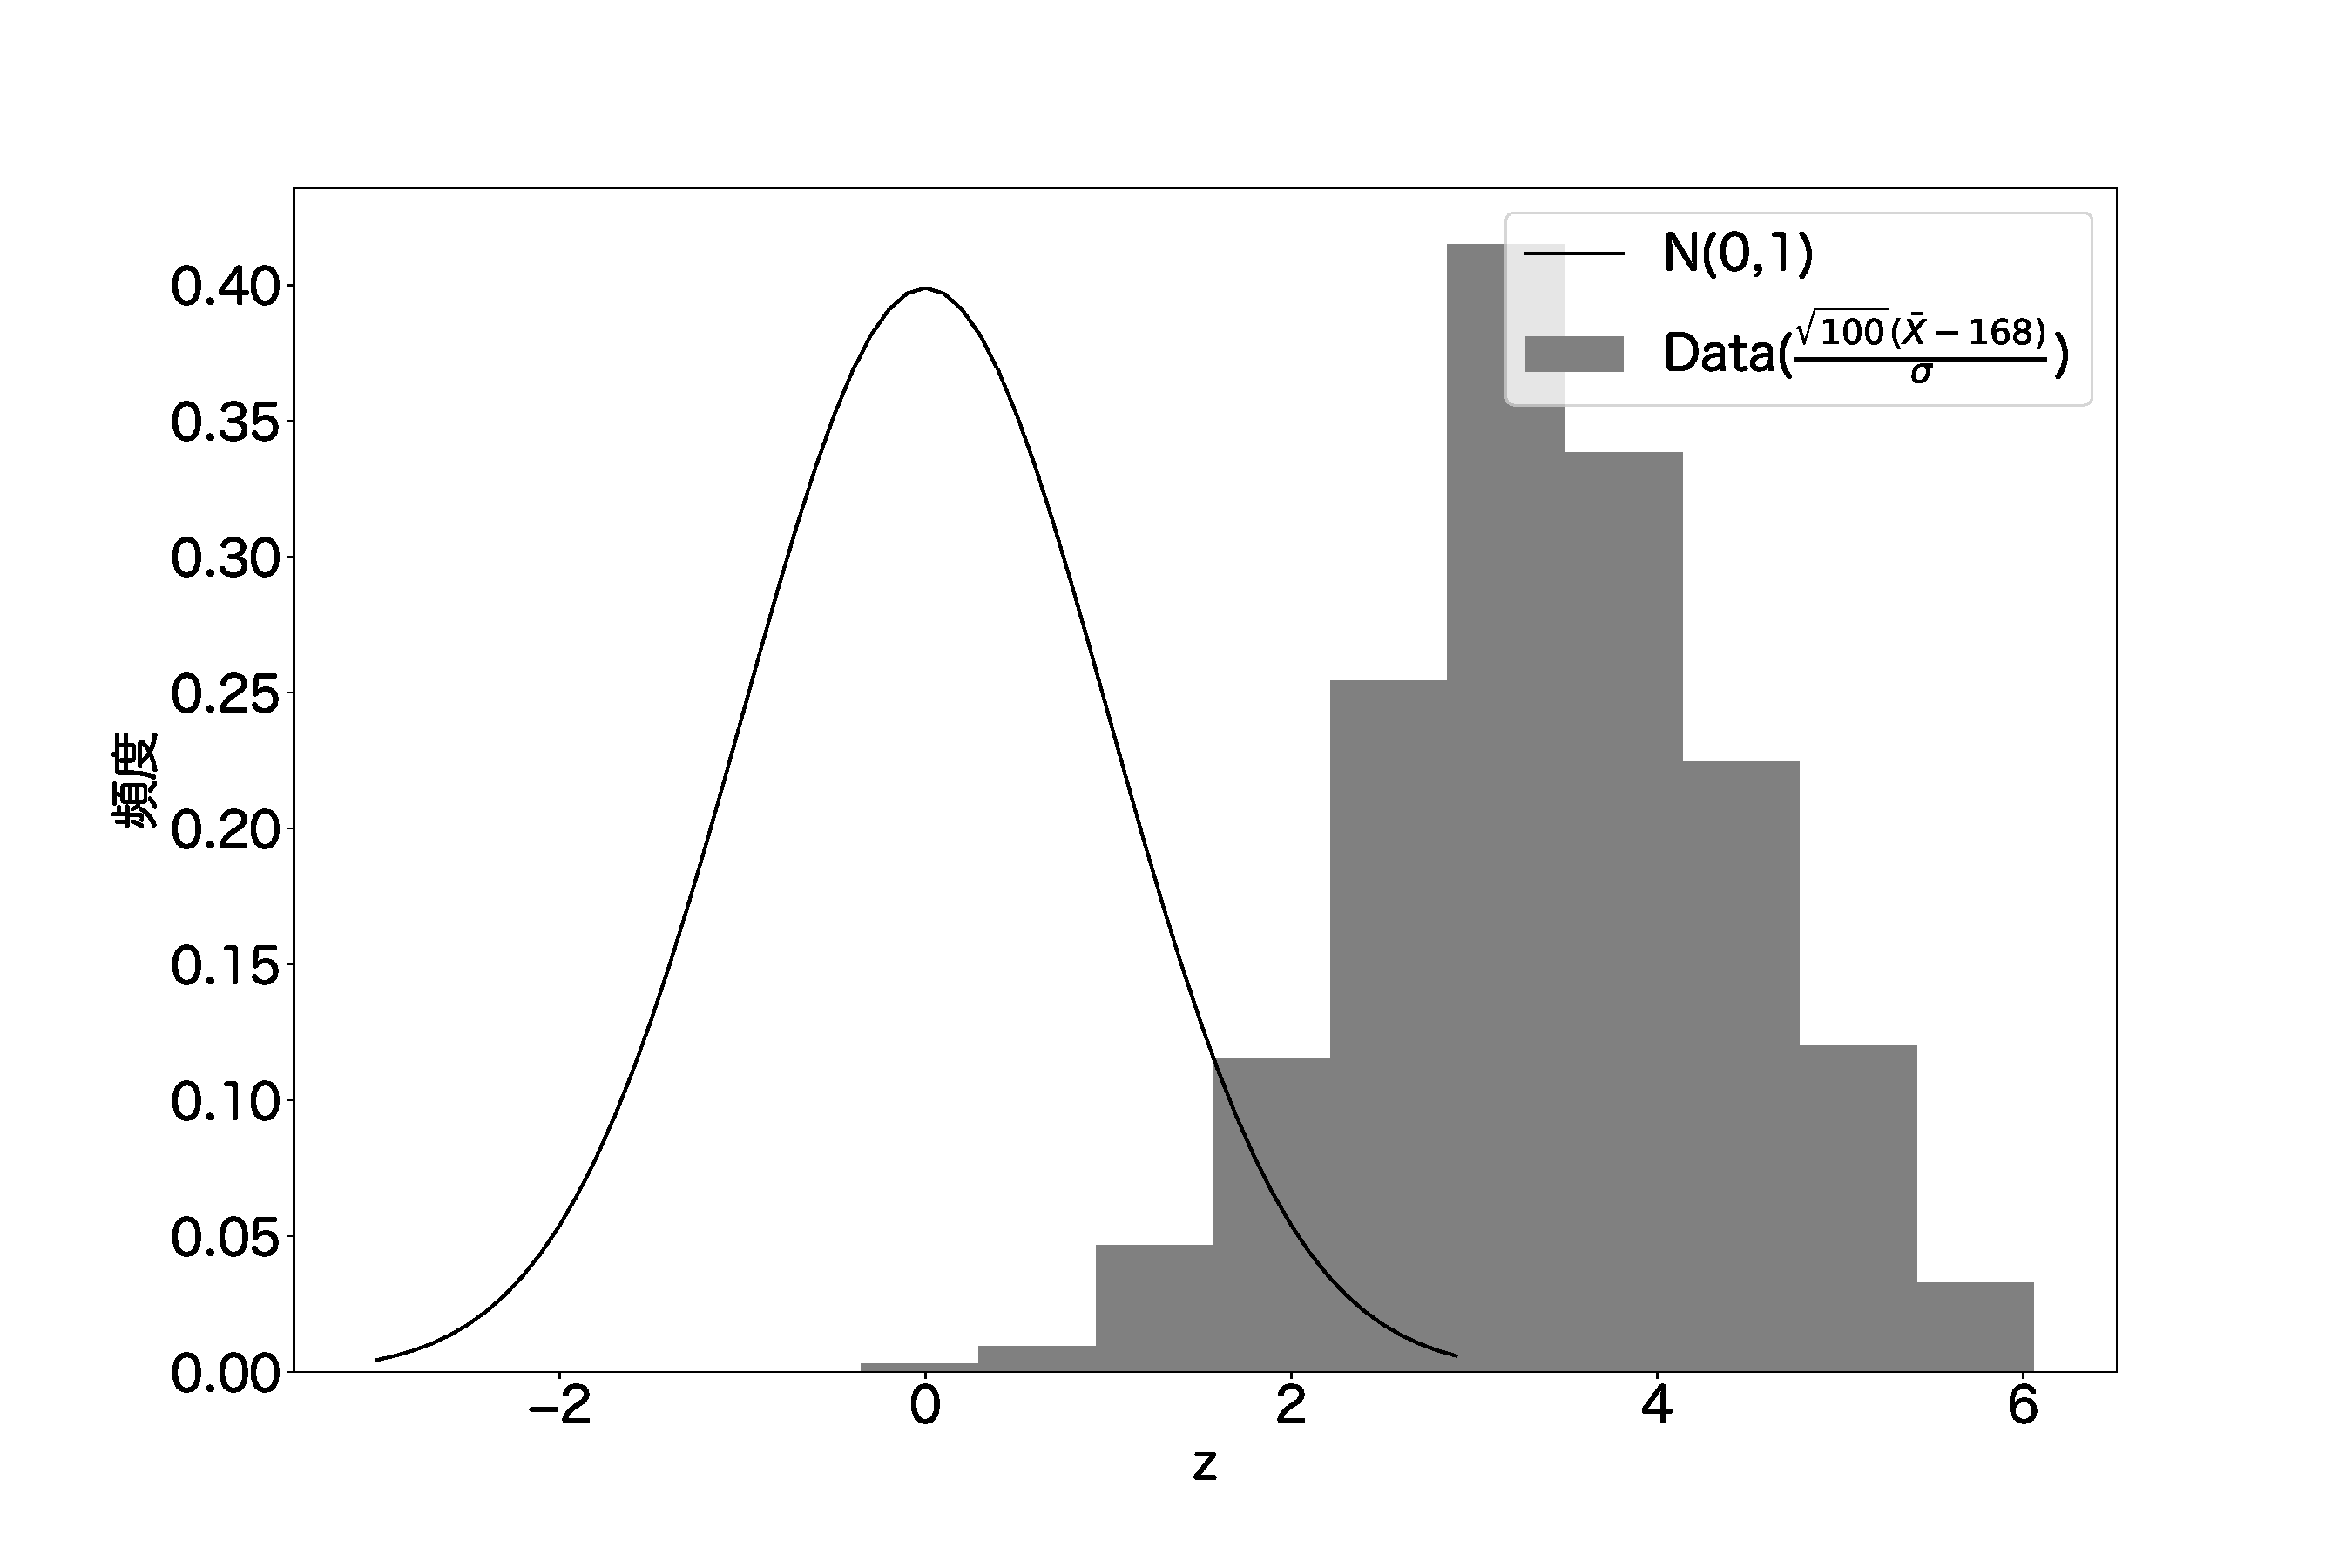
\includegraphics[width=15cm]{./image/02_/normal_distribution_test2.pdf}
        \caption{$N(170,5.8)$に従う確率変数を100個サンプリングし、その標本を1000個集めたときの$z=\sqrt{100}(\bar{X}-168)$のヒストグラム}
    \end{center}
\end{figure}


ある正規分布に従う確率変数$x_1,x_2,\cdots,x_n$が母数の異なる正規分布で得られる確率も計算できる。具体的には、$x_1,x_2,\cdots,x_n\sim N(\mu,\sigma^2)$とし、これが$N(\mu_1,\sigma_1^2)$で得られるとすると、そのときの統計量は、$z=\frac{\bar{x}-\mu_1}{\frac{\sigma_1}{n}}$である。この$z$は、$N(0,1)$に従うと考えられるので、$\phi(|z|>Z)$となる確率を計算すれば良い。

\begin{theo}
    確率変数$x_1,x_2,\cdots,x_n \sim N(\mu,\sigma^2)$ならば、$z=\frac{\bar{X}-\mu}{\sqrt{\frac{\sigma}{n}}} \sim N(0,1)$である。
    一方で、確率変数$x_1,x_2,\cdots,x_n \sim N(\mu,\sigma^2)$とする。$N(\mu_1,\sigma_1^2)$は正規分布とする。ただし、$\mu\neq \mu_1, \sigma =\sigma_1$このとき、$z=\frac{\bar{X}-\mu_1}{\sqrt{\frac{\sigma_1}{n}}} \sim N(0,1)$ではない。
\end{theo}
$\mu$と$ \mu_1$が極めて近い値のとき、$z=\frac{\bar{X}-\mu_1}{\sqrt{\frac{\sigma_1}{n}}} $も$N(0,1)$におけるよくある値になる言い換えれば、$\phi(|z|>Z)$は十分大きい。
一方で、$\mu$と$ \mu_1$が離れた値を取ると、$\phi(|z|>Z)$は小さな値になる。



\subsection{$(\star)$ $Exp(\lambda)$に従う確率変数であることを判定できるか}
$x_1,x_2,\cdots,x_n \sim Exp(\lambda)$であるとき、$n\bar{x}\sim Ga(n,\frac{1}{\lambda})$である。
母数不明の指数分布に従う確率変数が、$x_1,x_2,\cdots,x_n \sim Exp(\lambda)$と仮定したとき、$n\bar{x}\sim Ga(n,\frac{1}{\lambda})$でないならば、$x_1,x_2,\cdots,x_n \sim Exp(\lambda)$ではないと判断できるだろうか。シミュレーションによって確認してみよう。

この論法は、母数が不明の指数分布に従う確率変数を得たとき、その指数分布の母数が特定の値ではないことを示すためにこの論法を利用する。ここでは、母数が$\lambda=1,2,5,10,100$からサンプルサイズ4の標本を$1000$生成し、それら標本の統計量$n\bar{X}$のヒストグラムと、ガンマ関数$Ga(100,1)$の確率密度関数を比較する。

\begin{figure}
    \centering
    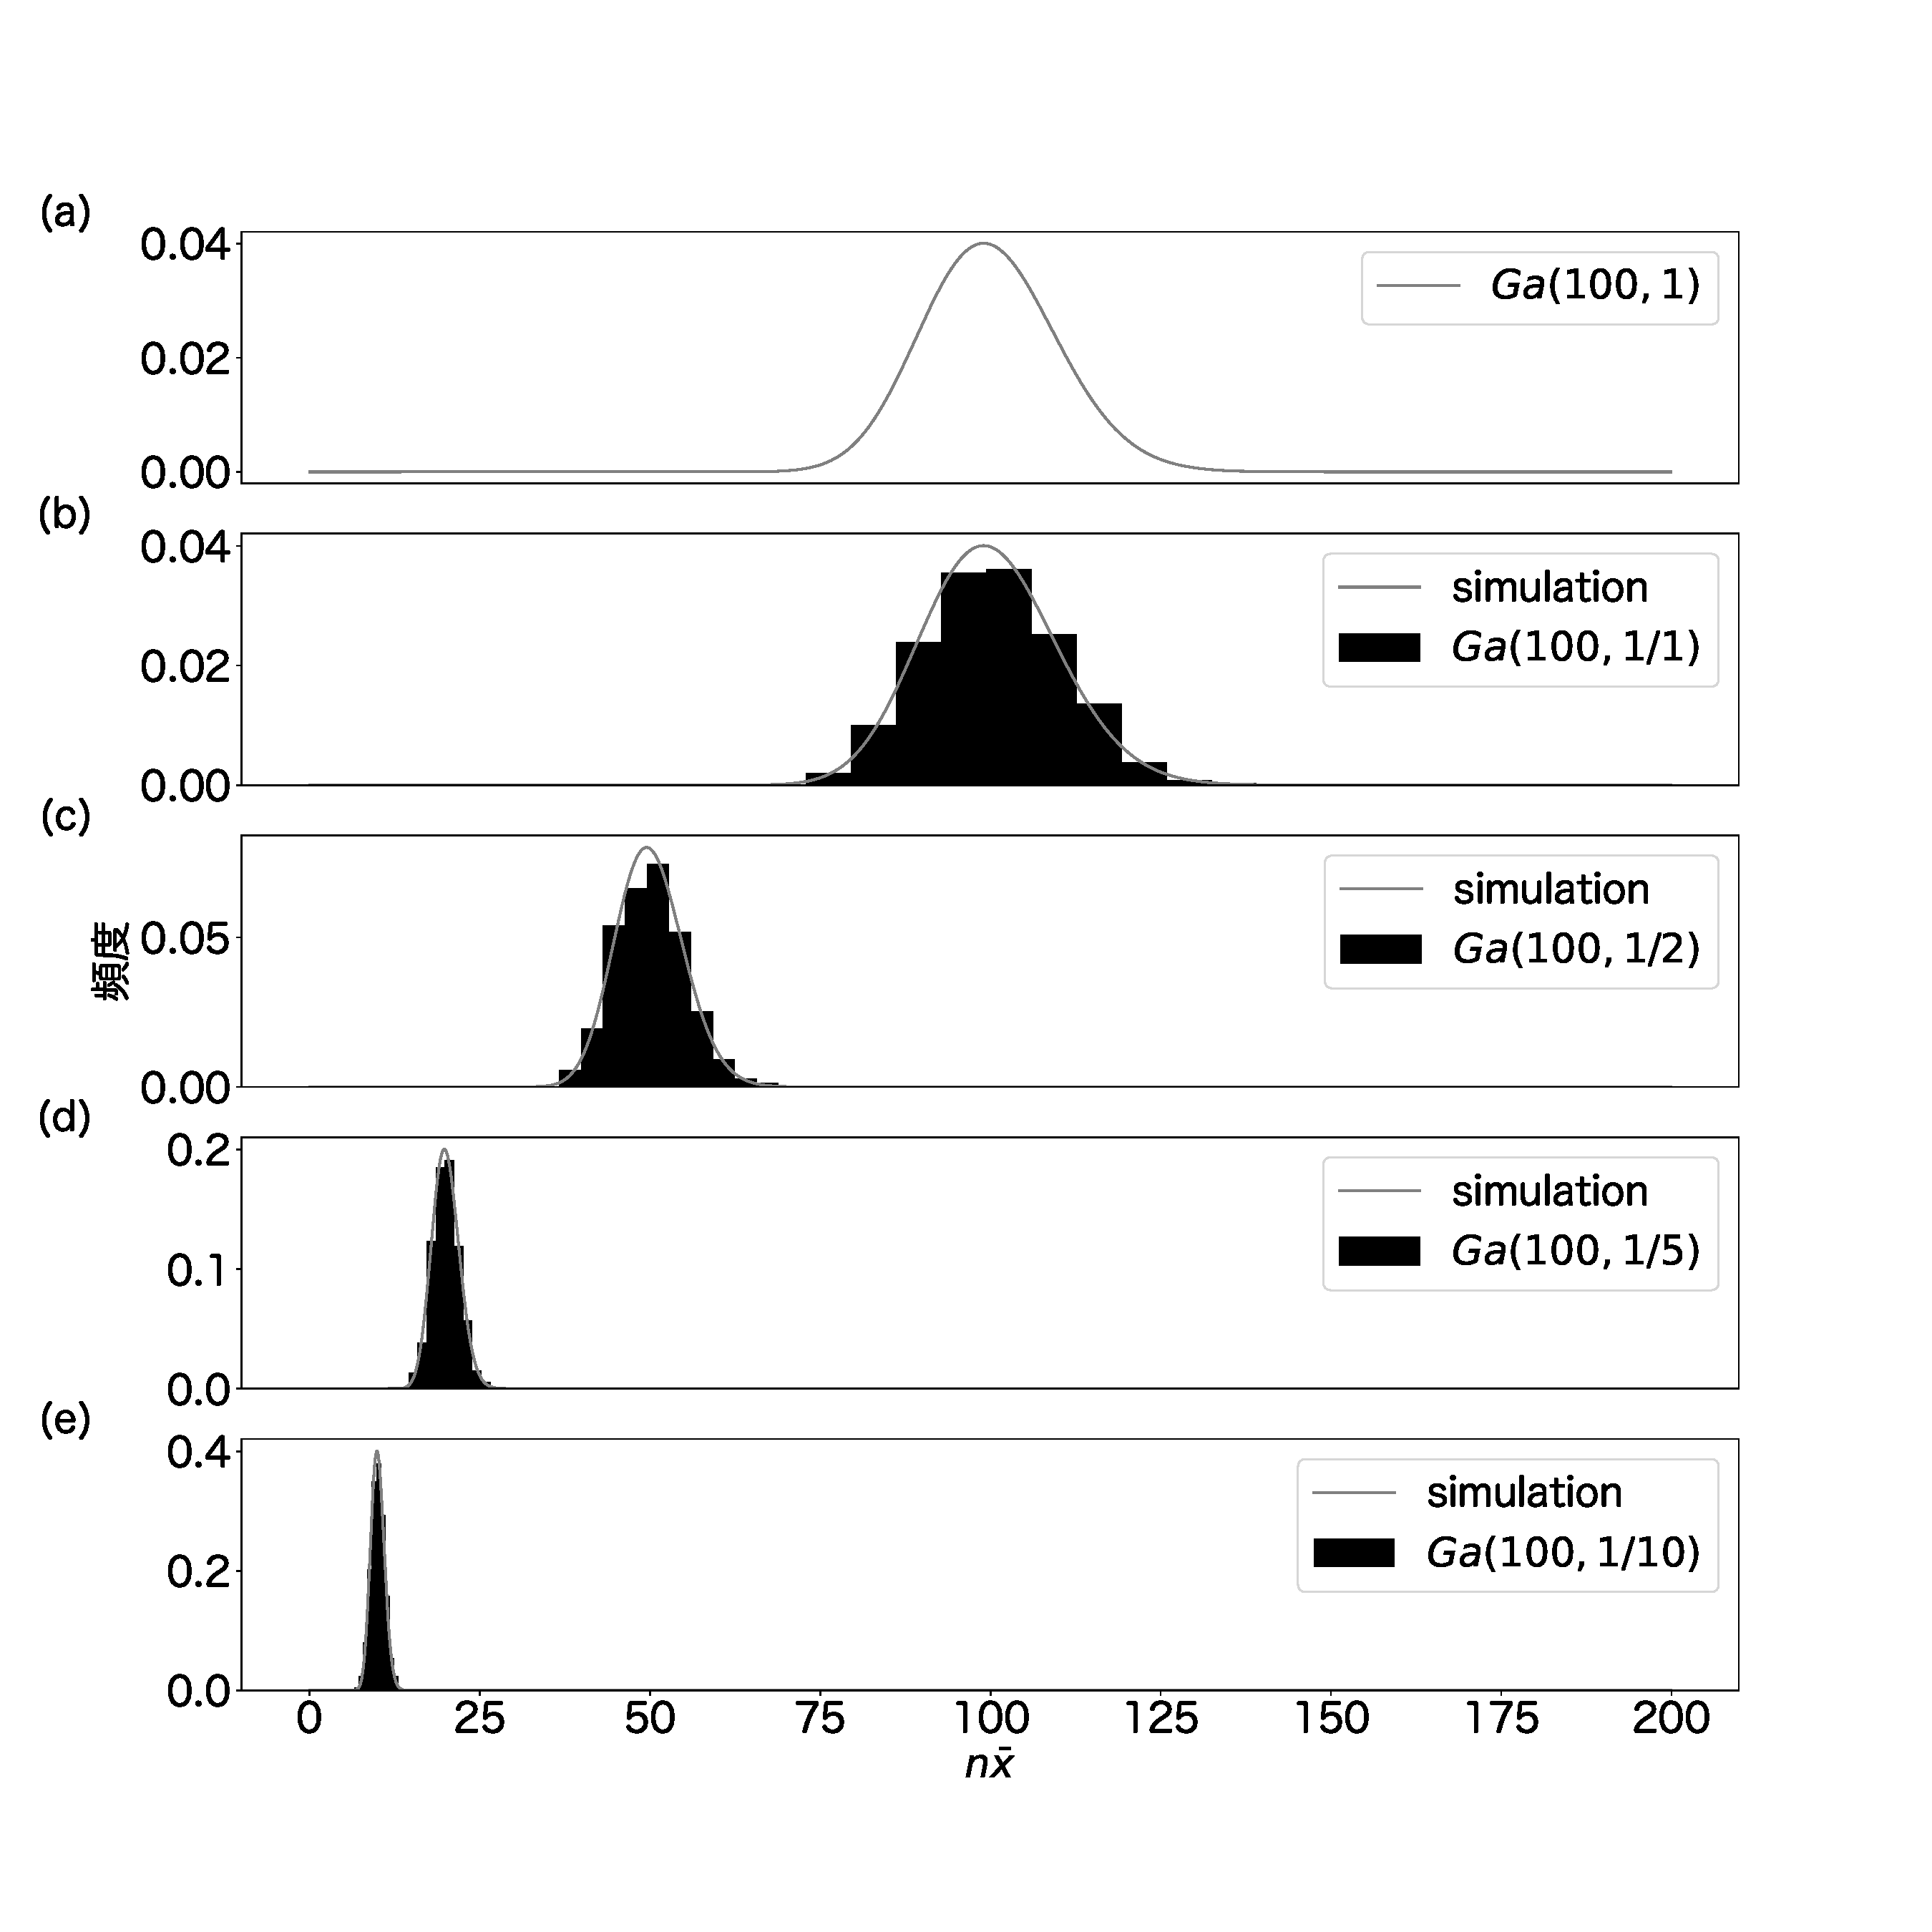
\includegraphics[width=15cm]{./image/02_/Exp_Gamma_simulation.pdf}
    \caption{(a)$Ga(10,1)$の確率密度関数。(b-e)指数分布からサンプルサイズ$4$の標本を$1000$回生成し、その統計量$n\bar{x}$のヒストグラム}
    \label{fig:exp_gamma_simulation}
\end{figure}

図\ref{fig:exp_gamma_simulation}(a)は、指数分布$Exp(\lambda=1)$の確率密度関数を示している。
図\ref{fig:exp_gamma_simulation}b-eは、シミュレーションの結果を示している。
図\ref{fig:exp_gamma_simulation}(b)には、指数分布$Exp(1)$に従う確率変数の統計量$n\bar{x}$が確かに、$Ga(100,1)$に従うことが確かめれる。
図\ref{fig:exp_gamma_simulation}(c-e)では、指数分布の$\lambda$が$1/2,1/5,1/10$のときの統計量のヒストグラムである。これらと、図\ref{fig:exp_gamma_simulation}(a)を比較すると、分布が異なっているので、確かに、$Ga(100,1)$には従わないことがわかる。



\subsection{TEST}

これらの事象は、統計モデルの上で観測される、数学的な事実です。
数学を扱っている以上はこの事実は決して崩れることはありえません。
一方で、我々が扱う現象ではどうなるでしょうか。現象が数学な分布関数から生成されていることは決してありえません。
誰かがサイコロを振って、人々の身長を決めているのなら話は別ですが、
人の身長が、ランダムに正規分布によって決定されることはありませんね。

$M(168)$モデルの平均値は$168cm$、データでは$171cm$程度なので、$3cm$小さい。また、
$180cm$以上の人の割合を使ってモデルとデータの乖離を調べることができました。
$180cm$の人がたまたまいなかった場合は、$M(169.1),M(168)$のどちらも推測できているとは言い難いことになります。このことから、特定の値を使って乖離を判定することは難しいと考えられます。


$\phi(z>Z(\mu))を$p値として、絶対に選択してはいけない統計モデル$M(\mu)$の母数$\mu$を調べます。具体的には、指標$p$が$0.05$より小さい統計モデルを選択しないようにします。その母数の範囲は$162.14 >\mu, \mu > 174.31$です。この母数の統計モデルは$p=0.05$の基準で使わないことを統計モデルを棄却すると言います。逆に、$p>0.05$となるモデルは、積極的に正しいとは考えません。明らかに間違いではないけども正しくもないという判断をします。


$p$値を使う方法がとられます。p値とは統計モデルとデータの乖離度合いを示す指標です。p値は$0~1$の値をとり、$0$に近いと統計モデルとデータが乖離していると判断します。




\section{04}
\subsubsection{いつでも正規モデルでいこう}
データが非対称に分布しているのに、統計モデルに正規分布を指定した場合、推定が正しく行えないことを確認しておこう\footnote{元ネタ。
    小標本 t 検定の誤解:中心極限定理と一般化線形モデル 井口豊(生物科学研究所,長野県岡谷市)\url{https://biolab.sakura.ne.jp/small-sample-t-test-glm.html}}。
次のような統計モデルを構築する。
\begin{enumerate}
    \item $X_1,X_2,\cdots,X_n $はi.i.d
    \item 正規分布
    \item 正規分布の母数$\mu$,$\sigma^2$の値は不明
\end{enumerate}
正規分布の母数$\mu=1$とした統計モデルを$M(1)$と記述する。
この$X_1,X_2,\cdots,X_n$について次の統計量が$t(n)$分布に従うことがわかっている。
\begin{equation*}
    T = \frac{\bar{X}-1}{\sqrt{\frac{\sigma^2}{n}}} \sim t(n)
\end{equation*}
このとき、データが、既知の確率分布から得られた場合に、$p$値がサンプルサイズによってどのように変化するのかを調べる。
具体的に、平均$1$の指数分布または、平均$1$、標準偏差$1$の正規分布からサンプルを得て標本を作る。その標本を$10^5$回取得する。
このとき、$T$値を計算し、$T$値いじょの値が得られる確率$p$を計算する。その$p$が$p<0.05$となる割合を計算する。以上をサンプルサイズを変化させてシミュレーションを行なった。

平均$1$、標準偏差$1$の正規分布の場合、統計モデルの仮定と一致するので、$T$値は$t(n)$分布に従う。よって、$p<0.05$となる頻度も、$5\%$程度になることが期待される。
一方で、平均$1$の指数分布の場合、統計モデルの仮定と一致しない。このことから、$T$は$t(n)$分布に従うとはいえない。このことから、$p<0.05$となる頻度はわからない。


\begin{figure}
    \begin{center}
        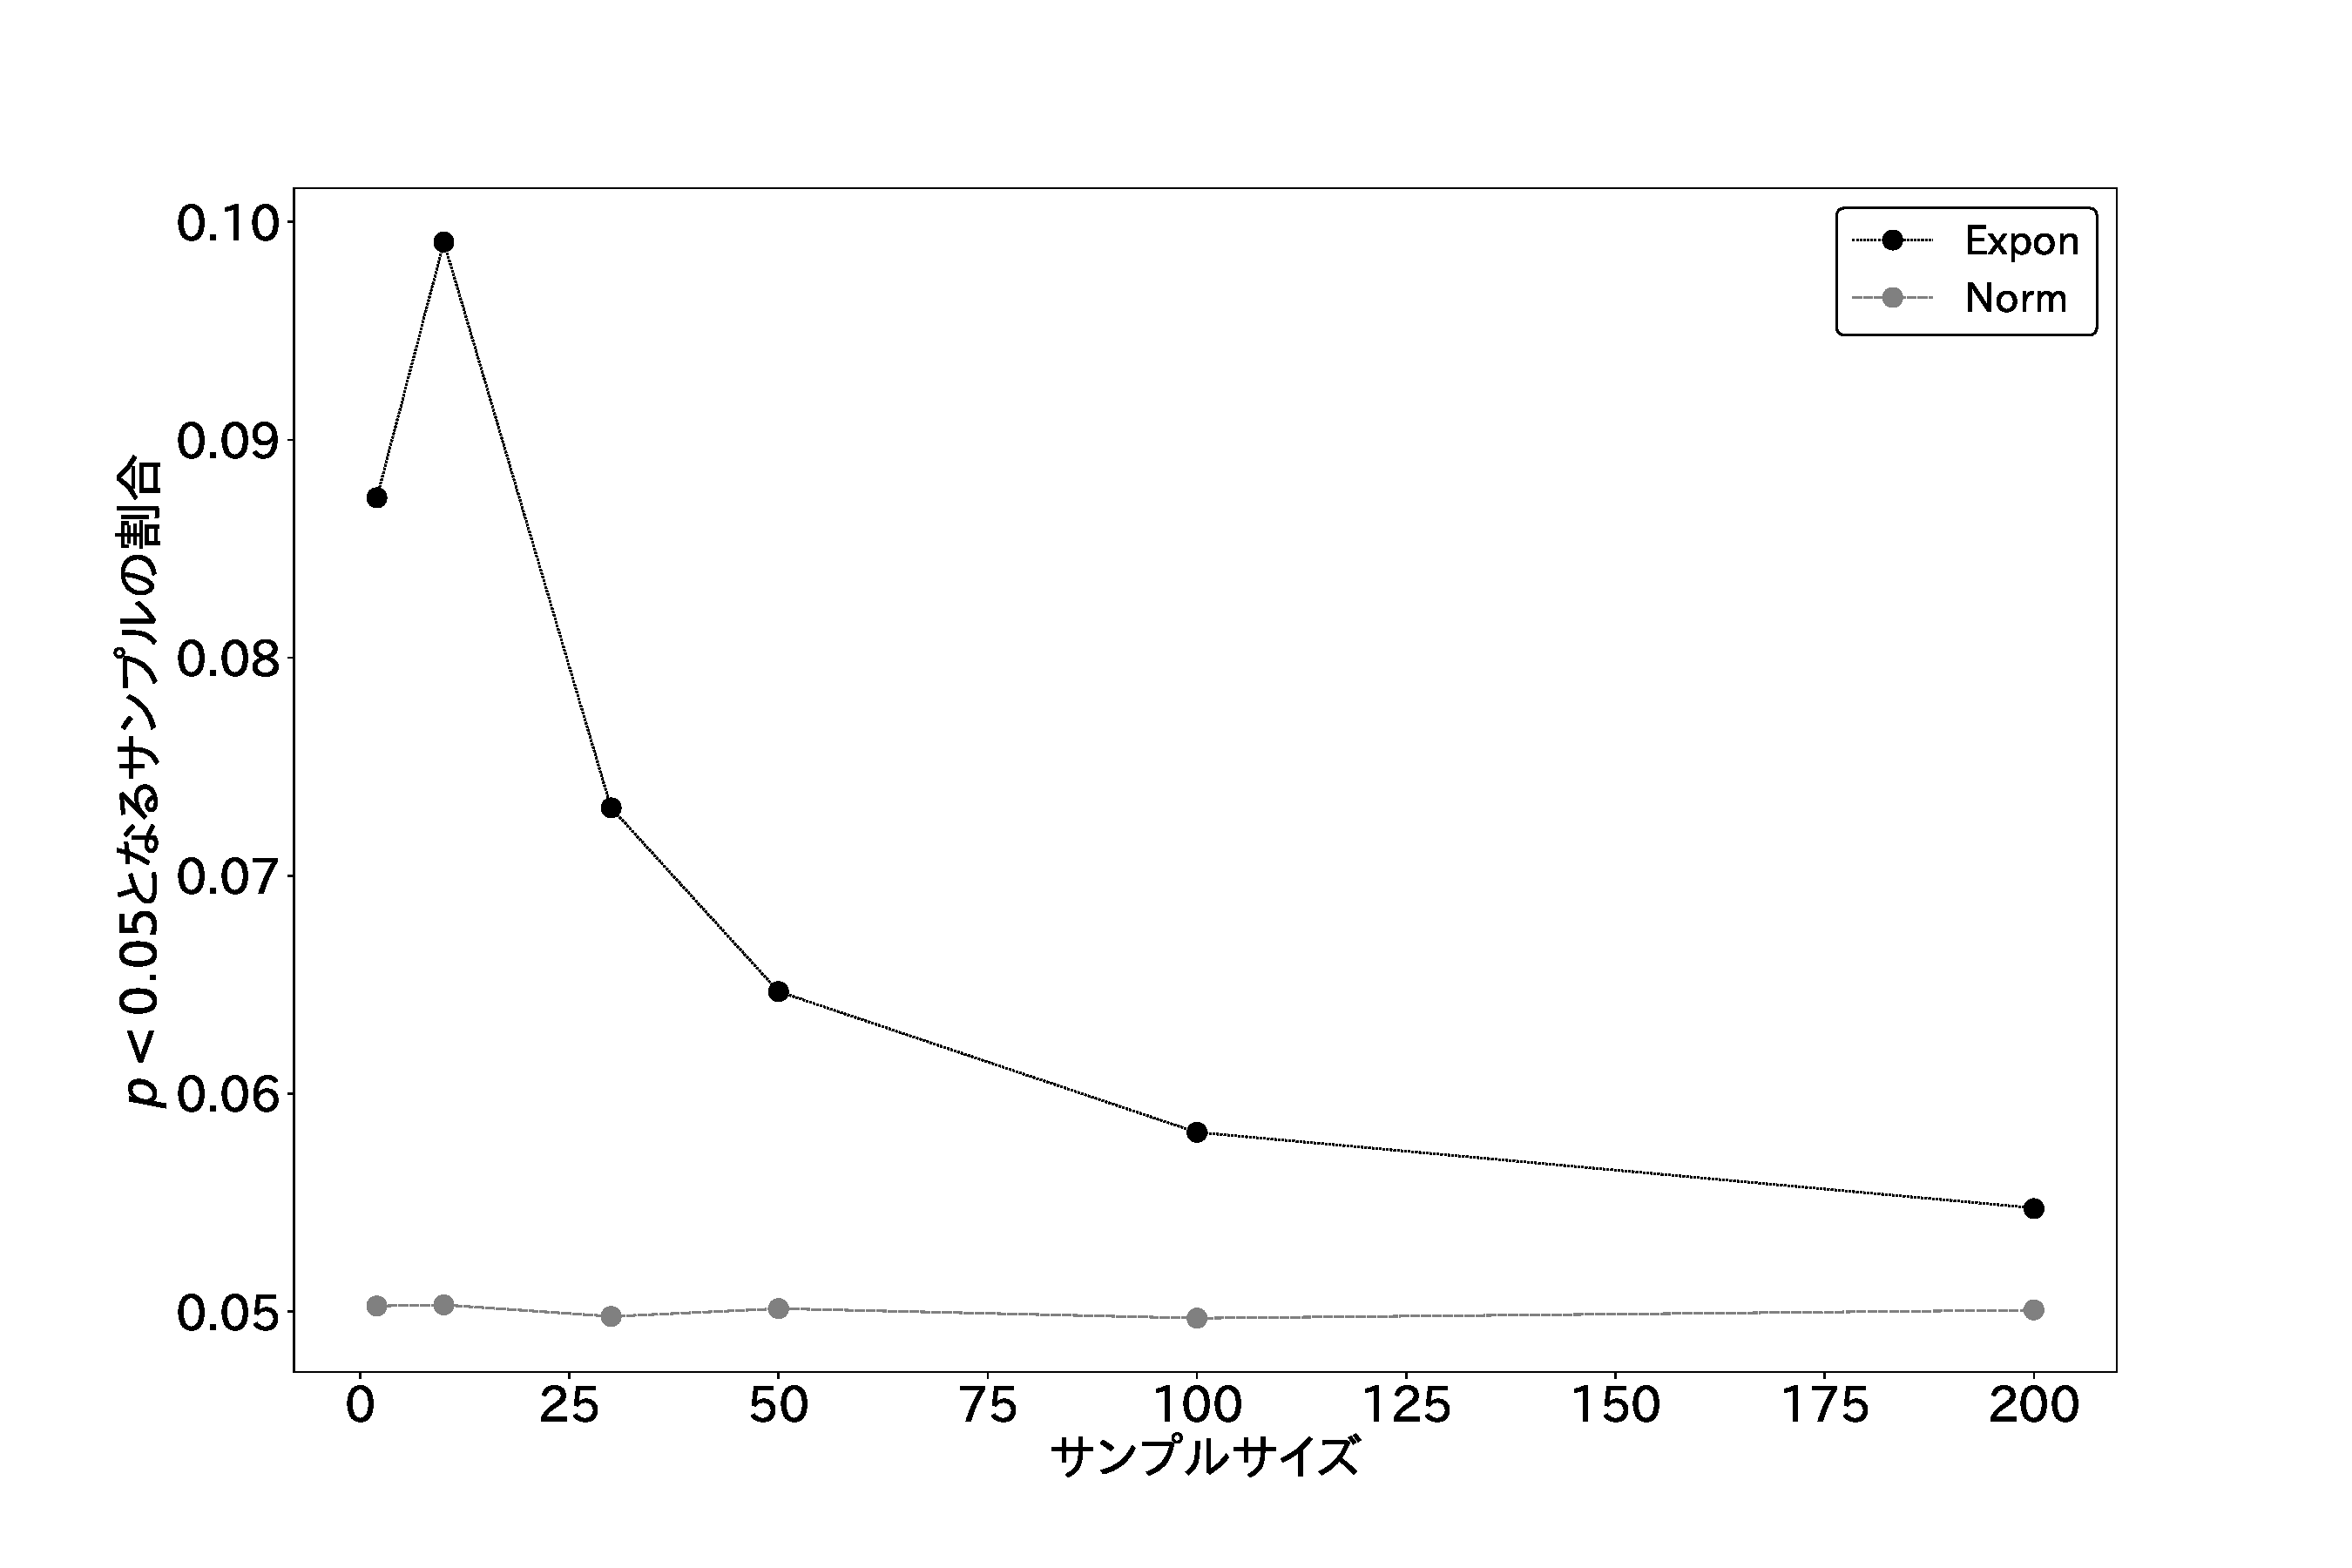
\includegraphics[width=15cm]{./image/04_/t_test_expon_norm.pdf}
        \caption{正規分布または指数ぶんぷから得た標本の$T$値から計算した$p$値で、$p<0.05$以下になる割合}
    \end{center}
\end{figure}

シミュレーションの結果、正規分布から標本を得た場合、$p<0.05$になる割合は、サンプルサイズに依存せず、$5\%$程度であり、理論と一致する。
一方で、指数分布から標本を得た場合、$p<0.05$になる割合はサンプルサイズに応じて変化しており、また、どのサンプルサイズでも$p<0.05$となる割合は$5\%$より多い。
このように、データが正規分布とかけ離れているにもかかわらず、正規モデルを構築し、そこから統計量を計算しても、的外れになることがあることを示唆している\footnote{$n$を大きくしたとき、中心極限定理より、$p<0.05$となる割合も$5\%$に近づくと解釈することがある。本当だろうか。具体的には、次の定理が成り立つのだろうか。
\begin{quote}
\begin{theo}
    $X_1,X_2,\cdots,X_n \sim Exp(\lambda)$とするとき、$T=\frac{\bar{X}-1/\lambda}{\sqrt{\frac{S^2}{n}}}$ここで、$S^2=\frac{1}{n-1}\sum_{i=1}^n(X_i-\bar{X})^2$である。$T\sim t(n-1)$または、$t$がなんらかの統計分布に従う。または、$E[T]<\infty,Var[T]<\infty$
\end{theo}
\end{quote}
このことが成り立つなら、中心極限定理も成立し、$n$が十分大きいときに、分布関数を近似できそうである。
}


\section{12}
\subsection{a}
このモデルにおいて、統計量$Z(\bar{x},\mu)$の$95\%$予測区間を求める。
%よく入る区間の式を変形し、データを得たときに、そのデータを基準にした$\mu$の範囲に変形してみます。
\begin{eqnarray*}
 & -z_{0.025} < Z(\bar{x},\mu)<z_{0.025} \\
\rightarrow & -z_{0.025} < \frac{\sqrt{n}(\bar{x}-\mu)}{\sigma}  <z_{0.025} \\
\rightarrow & \bar{x}- z_{0.025}\frac{\sigma}{\sqrt{n}} < \mu < \bar{x} + z_{0.025}\frac{\sigma}{\sqrt{n}}
\end{eqnarray*}


を使い、最尤モデルにおける平均値は、
$\bar{x}\sim N(\mu_{ML},\sigma^2_{ML}/\sqrt{n})$である。
このことから、モデルは、$\left[ \mu_{ML}-z_{0.05}\sigma_{ML},\mu_{ML}+z_{0.05}\sigma_{ML} \right]$
の間に、$68\%$の確率で平均値が入ることを予測する。


\begin{framed}
    まとめ、
    \begin{itemize}
        \item 統計モデル$M(\mu)$によってサンプリングし、標本を得たとき、標本平均値のよくある値の範囲が信頼区間
    \end{itemize}
    \end{framed}



    標本では、$168.9 < \mu < 176.0$、
この範囲にある$\mu$をもつ統計モデルであれば、この標本によって棄却されない。
%標本$2$では、$165.5 < \mu <172.6$です。
例えば、このモデル$M(\bar{x})$の信頼区間であれば、$M(168)$は棄却できない。




まとめ、
\begin{framed}
    \begin{itemize}
        \item 統計モデル$M(\mu)$のサンプルの平均が$95\%$の確率で入る範囲$\mu - z_{0.025} \frac{\sigma}{\sqrt{n}} < \bar{X} < \mu + z_{0.025} \frac{\sigma}{\sqrt{n}}$。現実の母集団が統計モデルによってよく推測できるなら、この範囲に平均値が入る確率は$95\%$に近くなることもある。逆に、統計モデルが現実をよく捉えることができなければ、母集団から無作為抽出した標本の平均値はこの範囲に入ることは少なくなる。
        \item データがよくある範囲に入る統計モデル$M(\mu)$の$\mu$の範囲$\bar{x}- z_{0.025}\frac{\sigma}{\sqrt{n}} < \mu < \bar{x} + z_{0.025}\frac{\sigma}{\sqrt{n}}$
        \item  統計モデル$M(\mu)$ではサンプルサイズを大きくすると、平均値が入る範囲が狭くなる。
    \end{itemize}
\end{framed}


複数の確率変数$x_1,x_2,\cdots,x_n$が$N(\mu,\sigma^2)$に従わないことを推定したい。

サンプルサイズが大きいときは、最尤推定を行い、$\mu_1=\bar{x},\sigma_1^2=\sum_{i=1}^{n} (x_i-\bar{x})^2/n$を計算し、その値が、$\mu,\sigma^2$と著しく異なっていれば、$N(\mu,\sigma^2)$に従わないと言えそうである。
例えば、図\ref{fig:maximum_likelihood_0}は、正規分布$N(170,6.8^2)$からサンプルサイズ$100$の標本を得たとき、図\ref{fig:maximum_likelihood_1}は、サンプルサイズ$30$、そしてそのデータの分布と、最尤推定量から予測されるも確率密度関数、$N(168,6.8^2),N(171,6.8^2)$を表している。図\ref{fig:maximum_likelihood_0}をみると、最尤推定した確率密度関数がデータの出現頻度をよく表していること、そして、周辺の二つの正規分布$N(168,6.8^2),N(171,6.8^2)$とデータが乖離していることがわかる。
一方、図\ref{fig:maximum_likelihood_1}では、データが$N(171,6.8^2)$に従っているのではないかという疑惑が残る。

\begin{figure}
    \begin{center}
        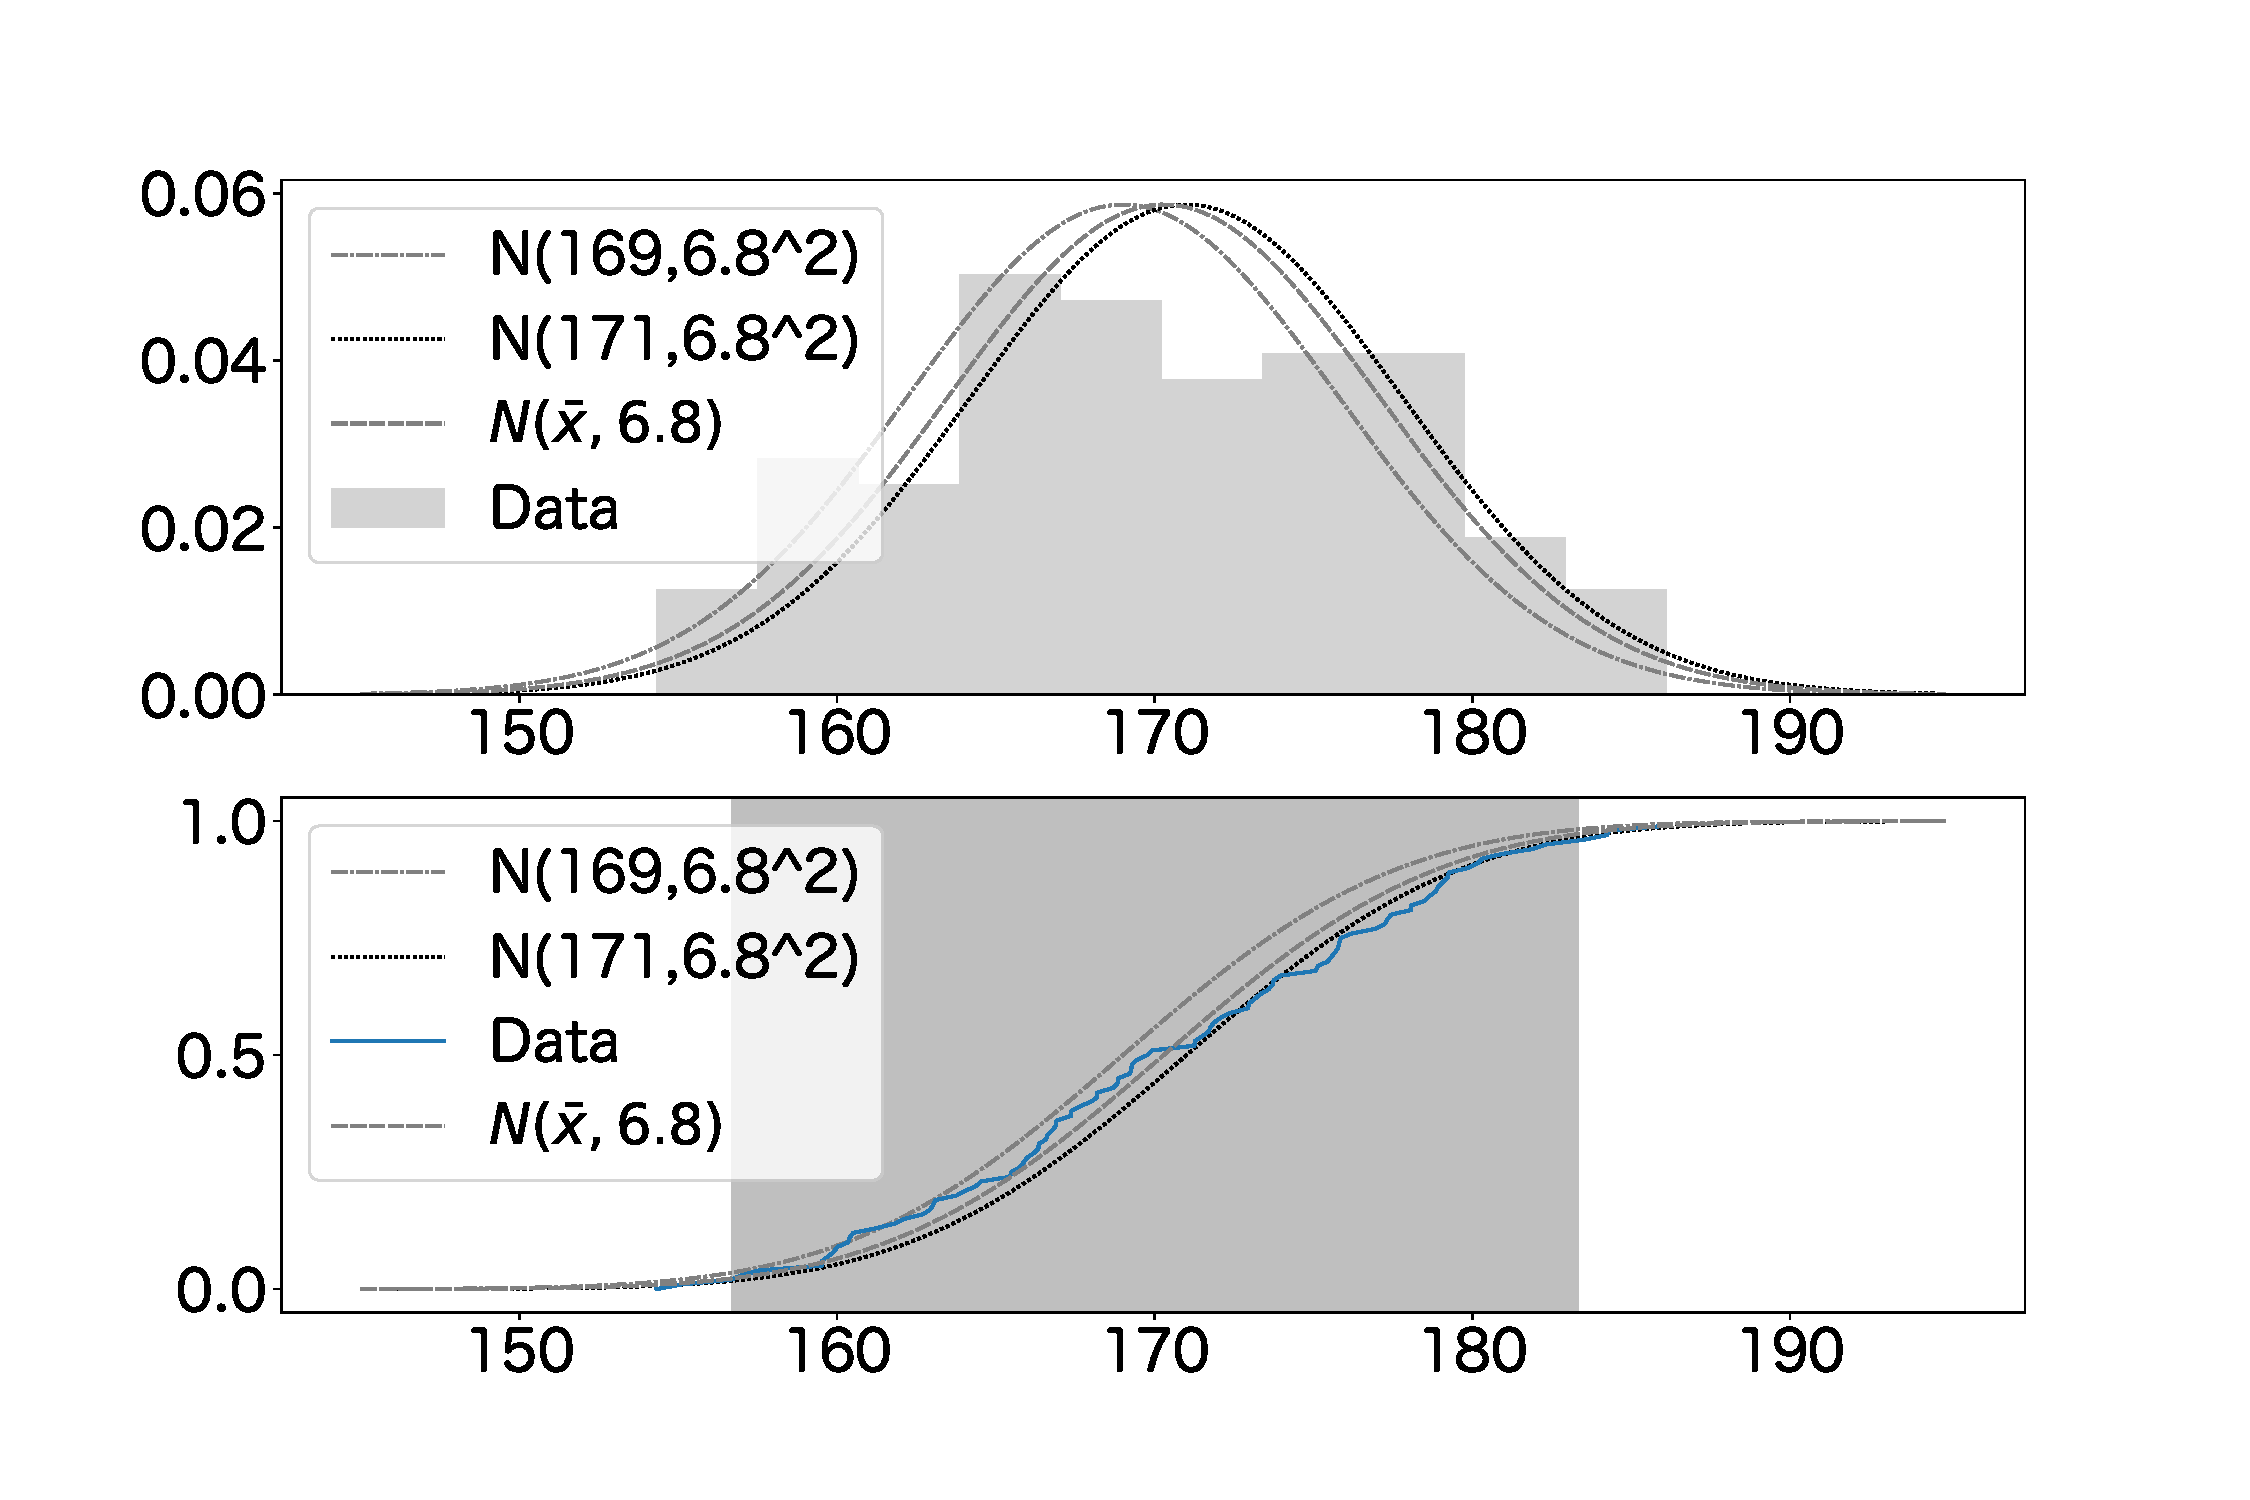
\includegraphics[width=15cm]{./image/02_/maximum_likelihood_0.pdf}
        \caption{$N(170,6.8^2)$からサンプルサイズ$100$の標本を得たときの分布。その最尤推定量により求められる分布関数。$N(168,6.8^2),N(171,6.8^2)$の分布関数を示す}
        \label{fig:maximum_likelihood_0}
    \end{center}
\end{figure}
\begin{figure}
    \begin{center}
        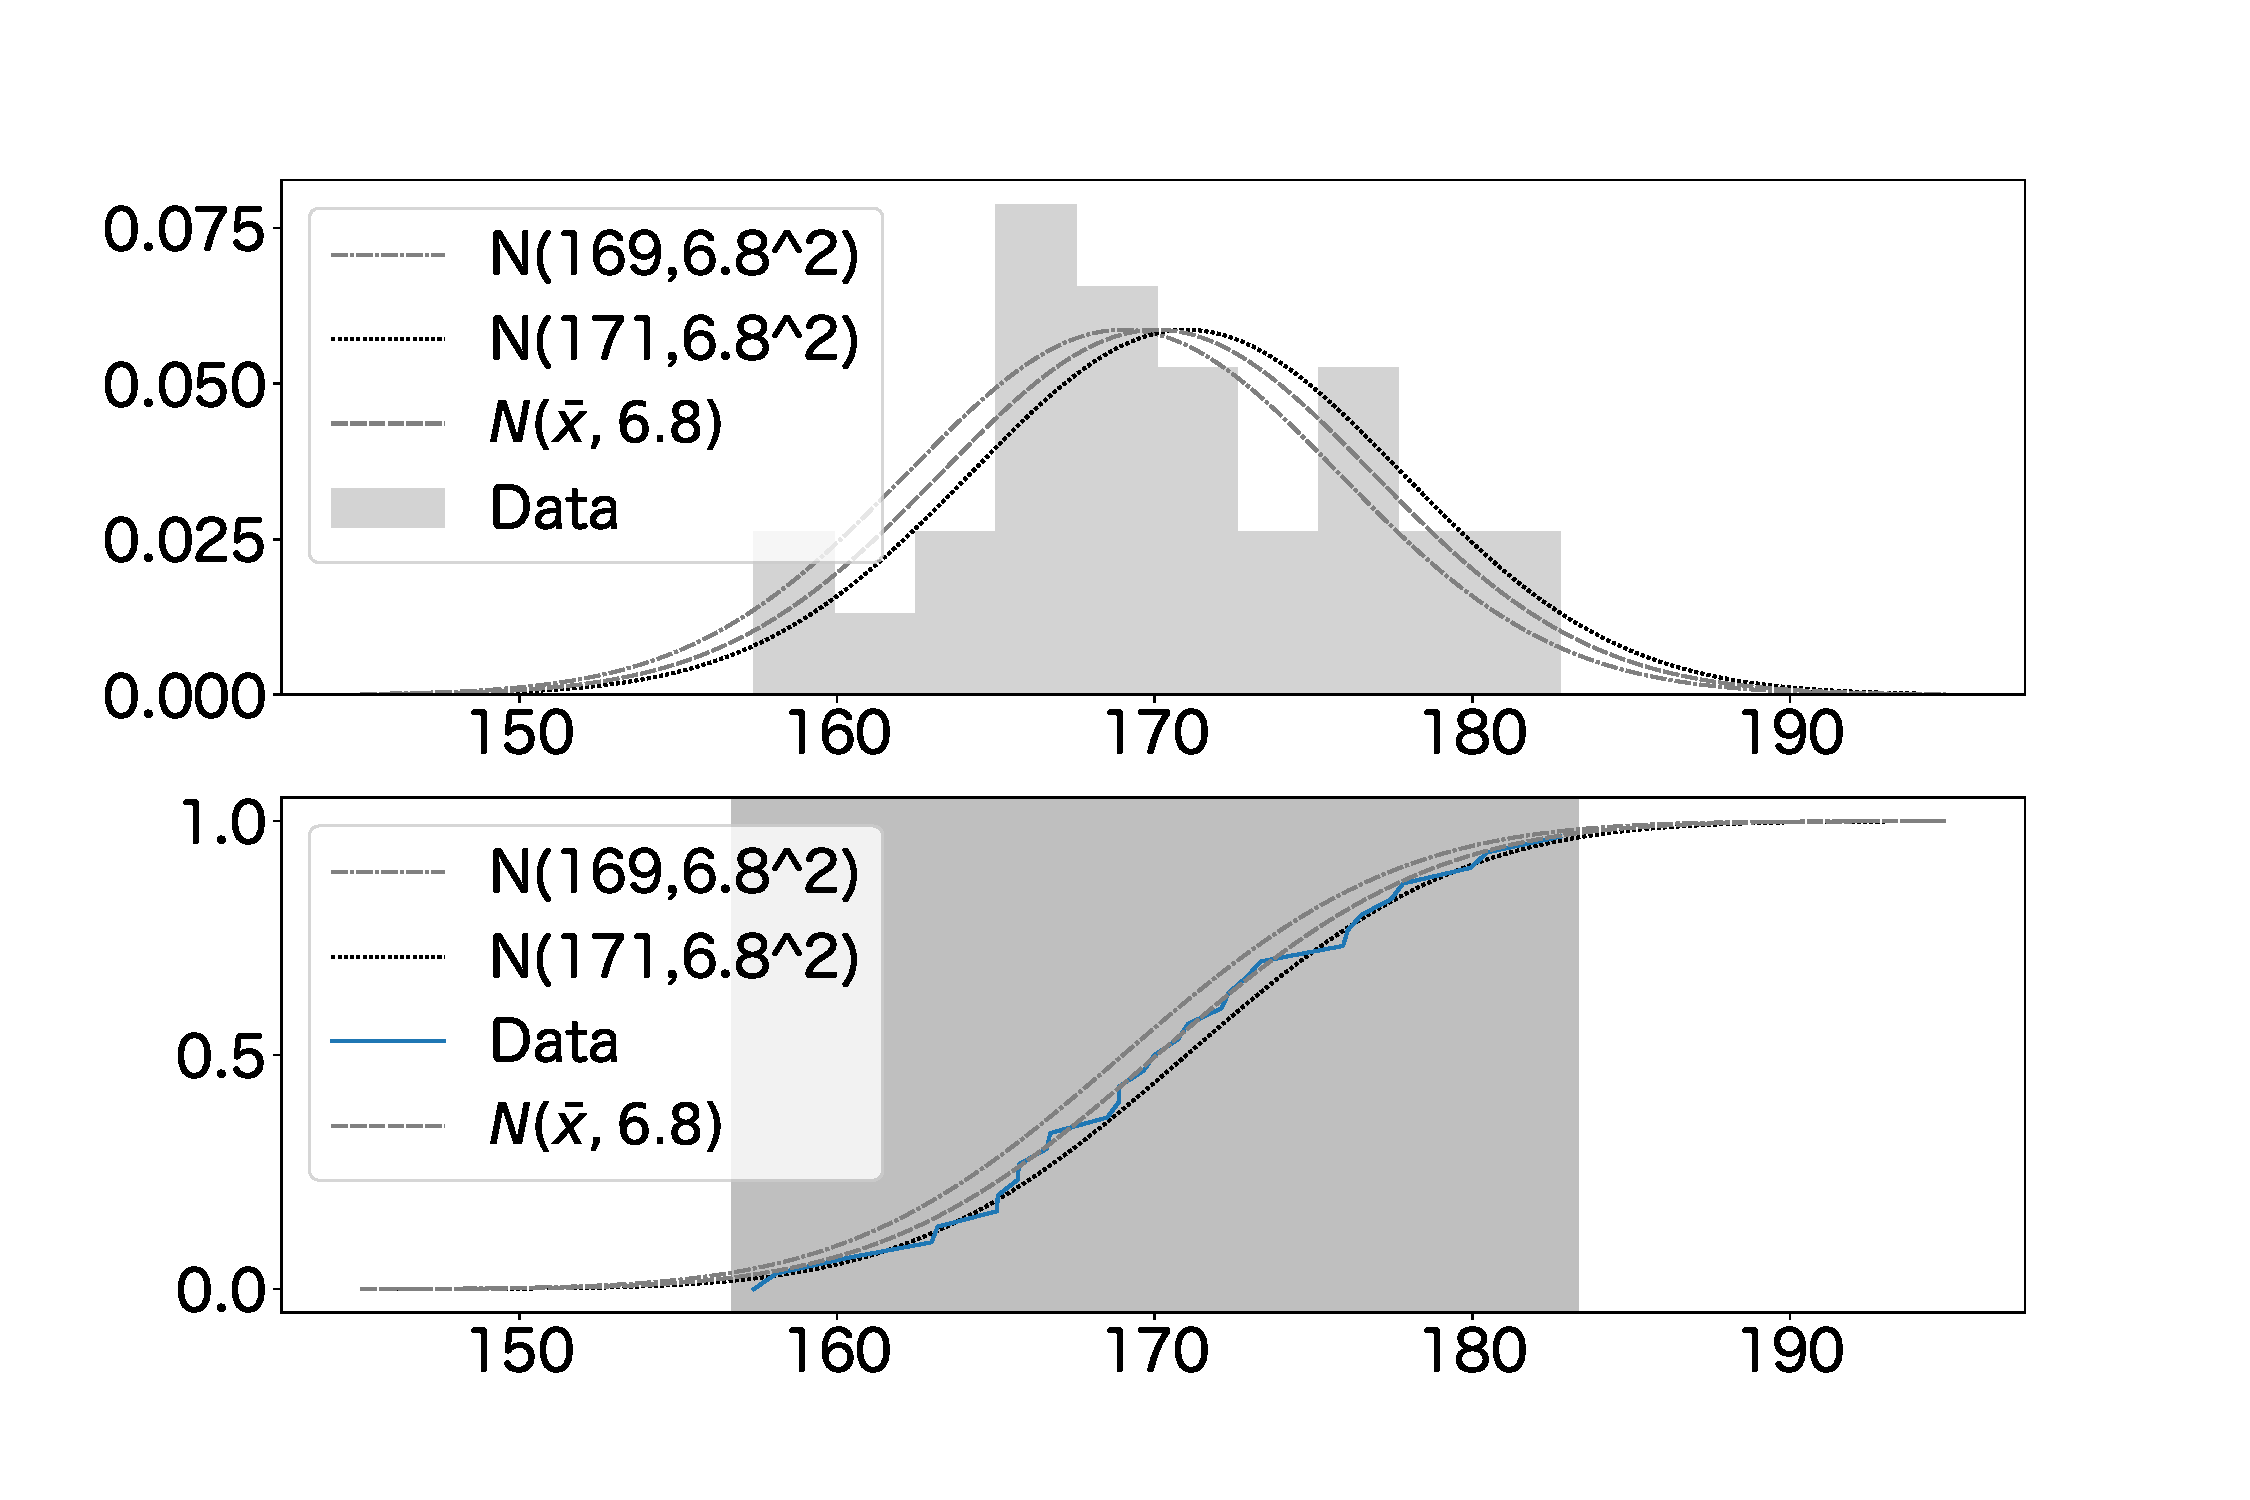
\includegraphics[width=15cm]{./image/02_/maximum_likelihood_1.pdf}
        \caption{$N(170,6.8^2)$からサンプルサイズ$30$の標本を得たときの分布。その最尤推定量により求められる分布関数。$N(168,6.8^2),N(171,6.8^2)$の分布関数を示す}
        \label{fig:maximum_likelihood_1}
    \end{center}
\end{figure}

このように、サンプルサイズが大きいと、最尤推定により推測した確率密度関数を見れば、そのほかの母数に従わないことがわかる場合がある。
また、より近くにある母数の確率密度関数と区別することは難しいこともわかる。

\begin{figure}
    \begin{center}
        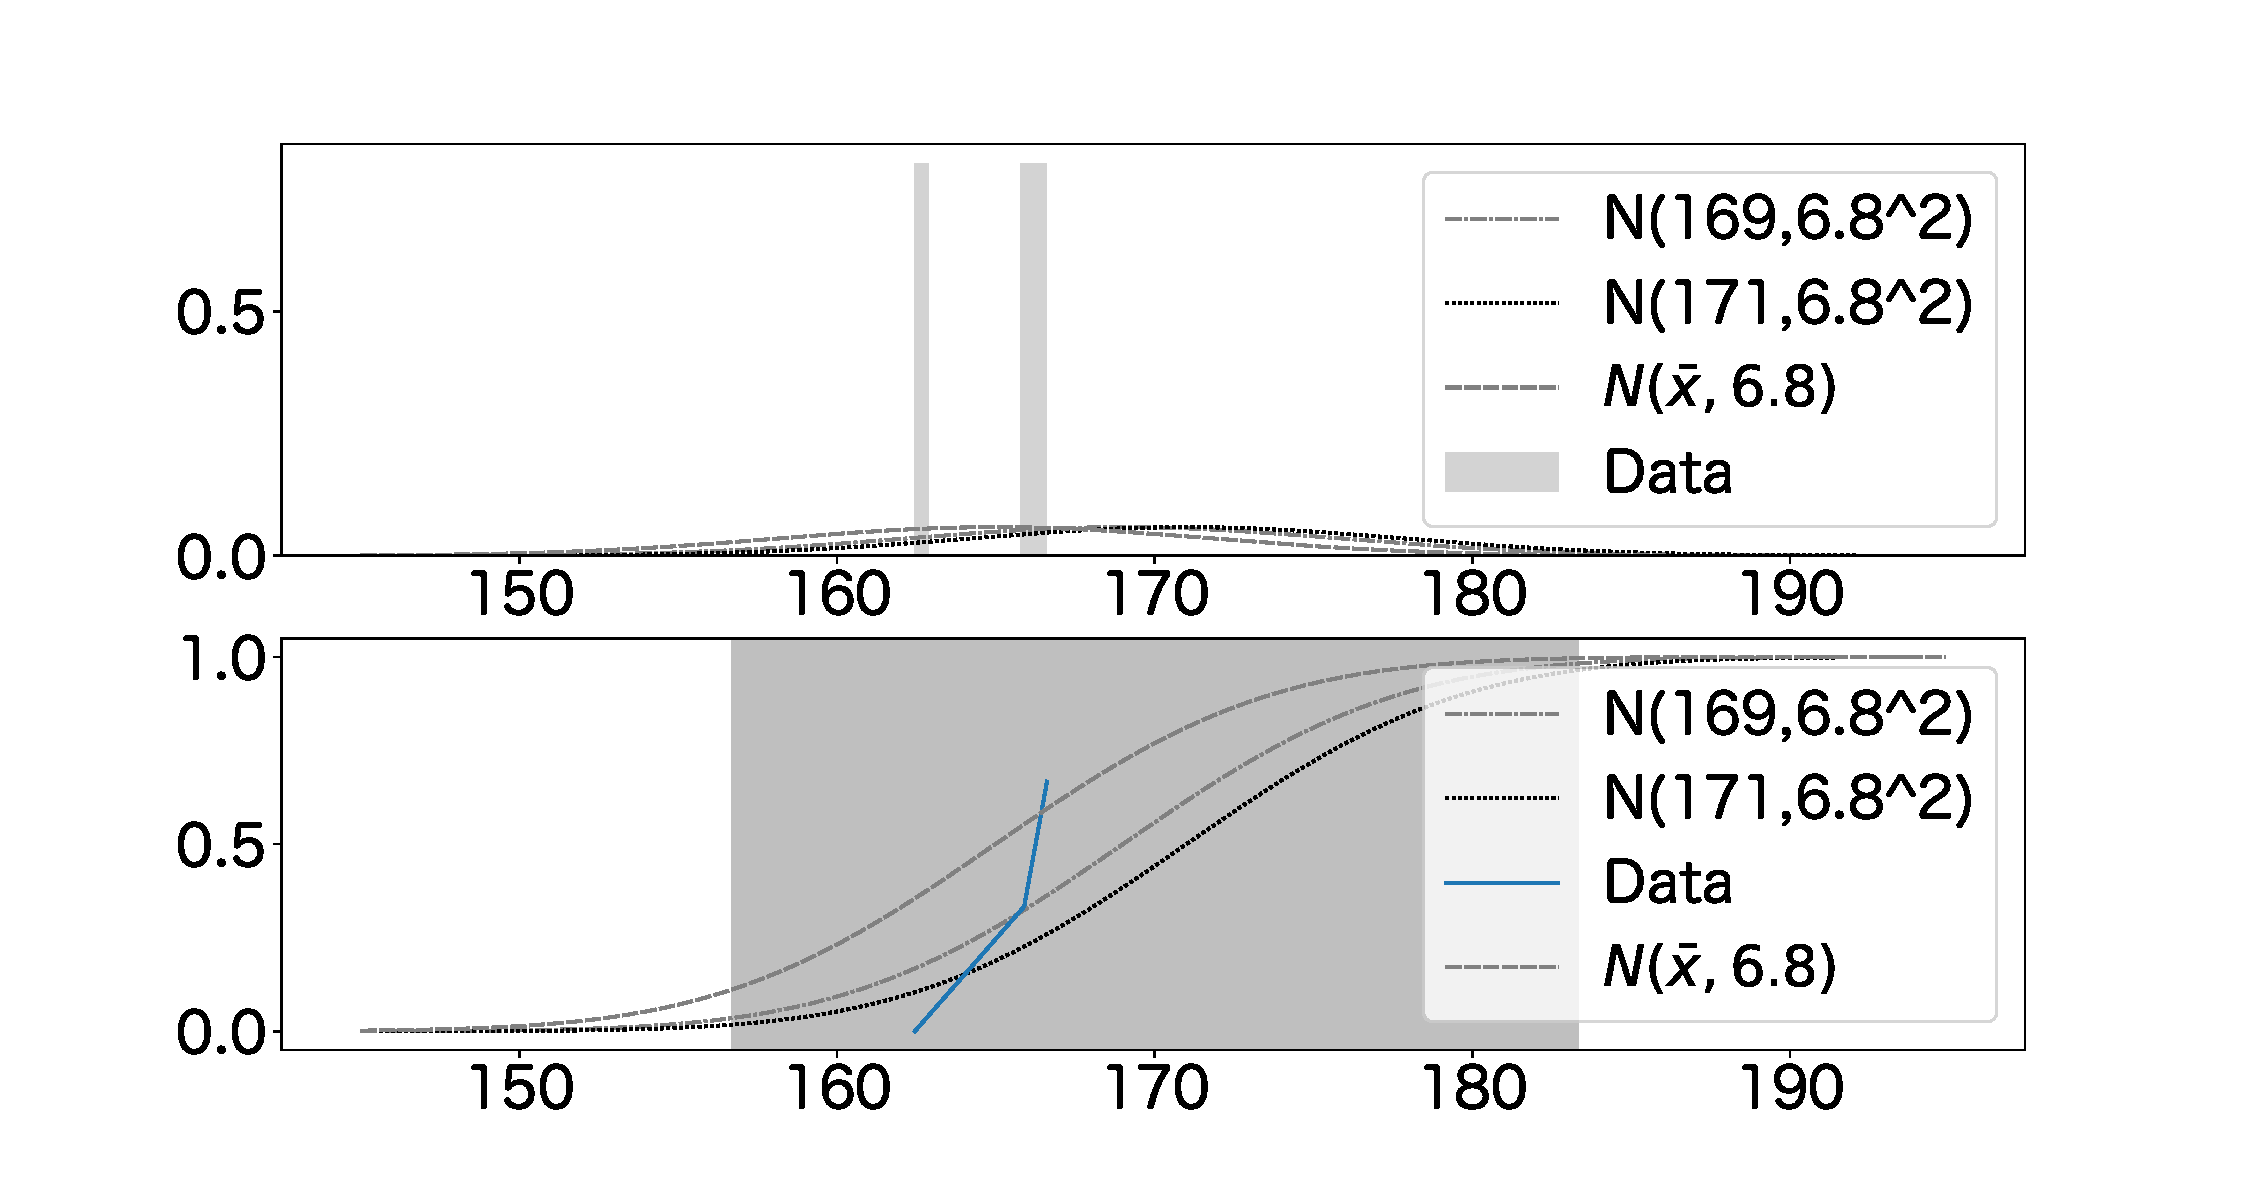
\includegraphics[width=15cm]{./image/02_/maximum_likelihood_3.pdf}
        \caption{$N(170,6.8^2)$からサンプルサイズ$3$の標本を得たときの分布。その最尤推定量により求められる分布関数。$N(168,6.8^2),N(171,6.8^2)$の分布関数を示す}
        \label{fig:maximum_likelihood_0}
    \end{center}
\end{figure}




\subsection{全然違うはなんとなくわかる}
図\ref{fig:maximum_likelihood_false_3},\ref{fig:maximum_likelihood_false_30}は、$N(170,6.8^2)$からサンプリングしたデータの度数分布と、その確率密度関数とは著しく異なる確率密度関数を表示したものです。

\begin{figure}
    \begin{center}
        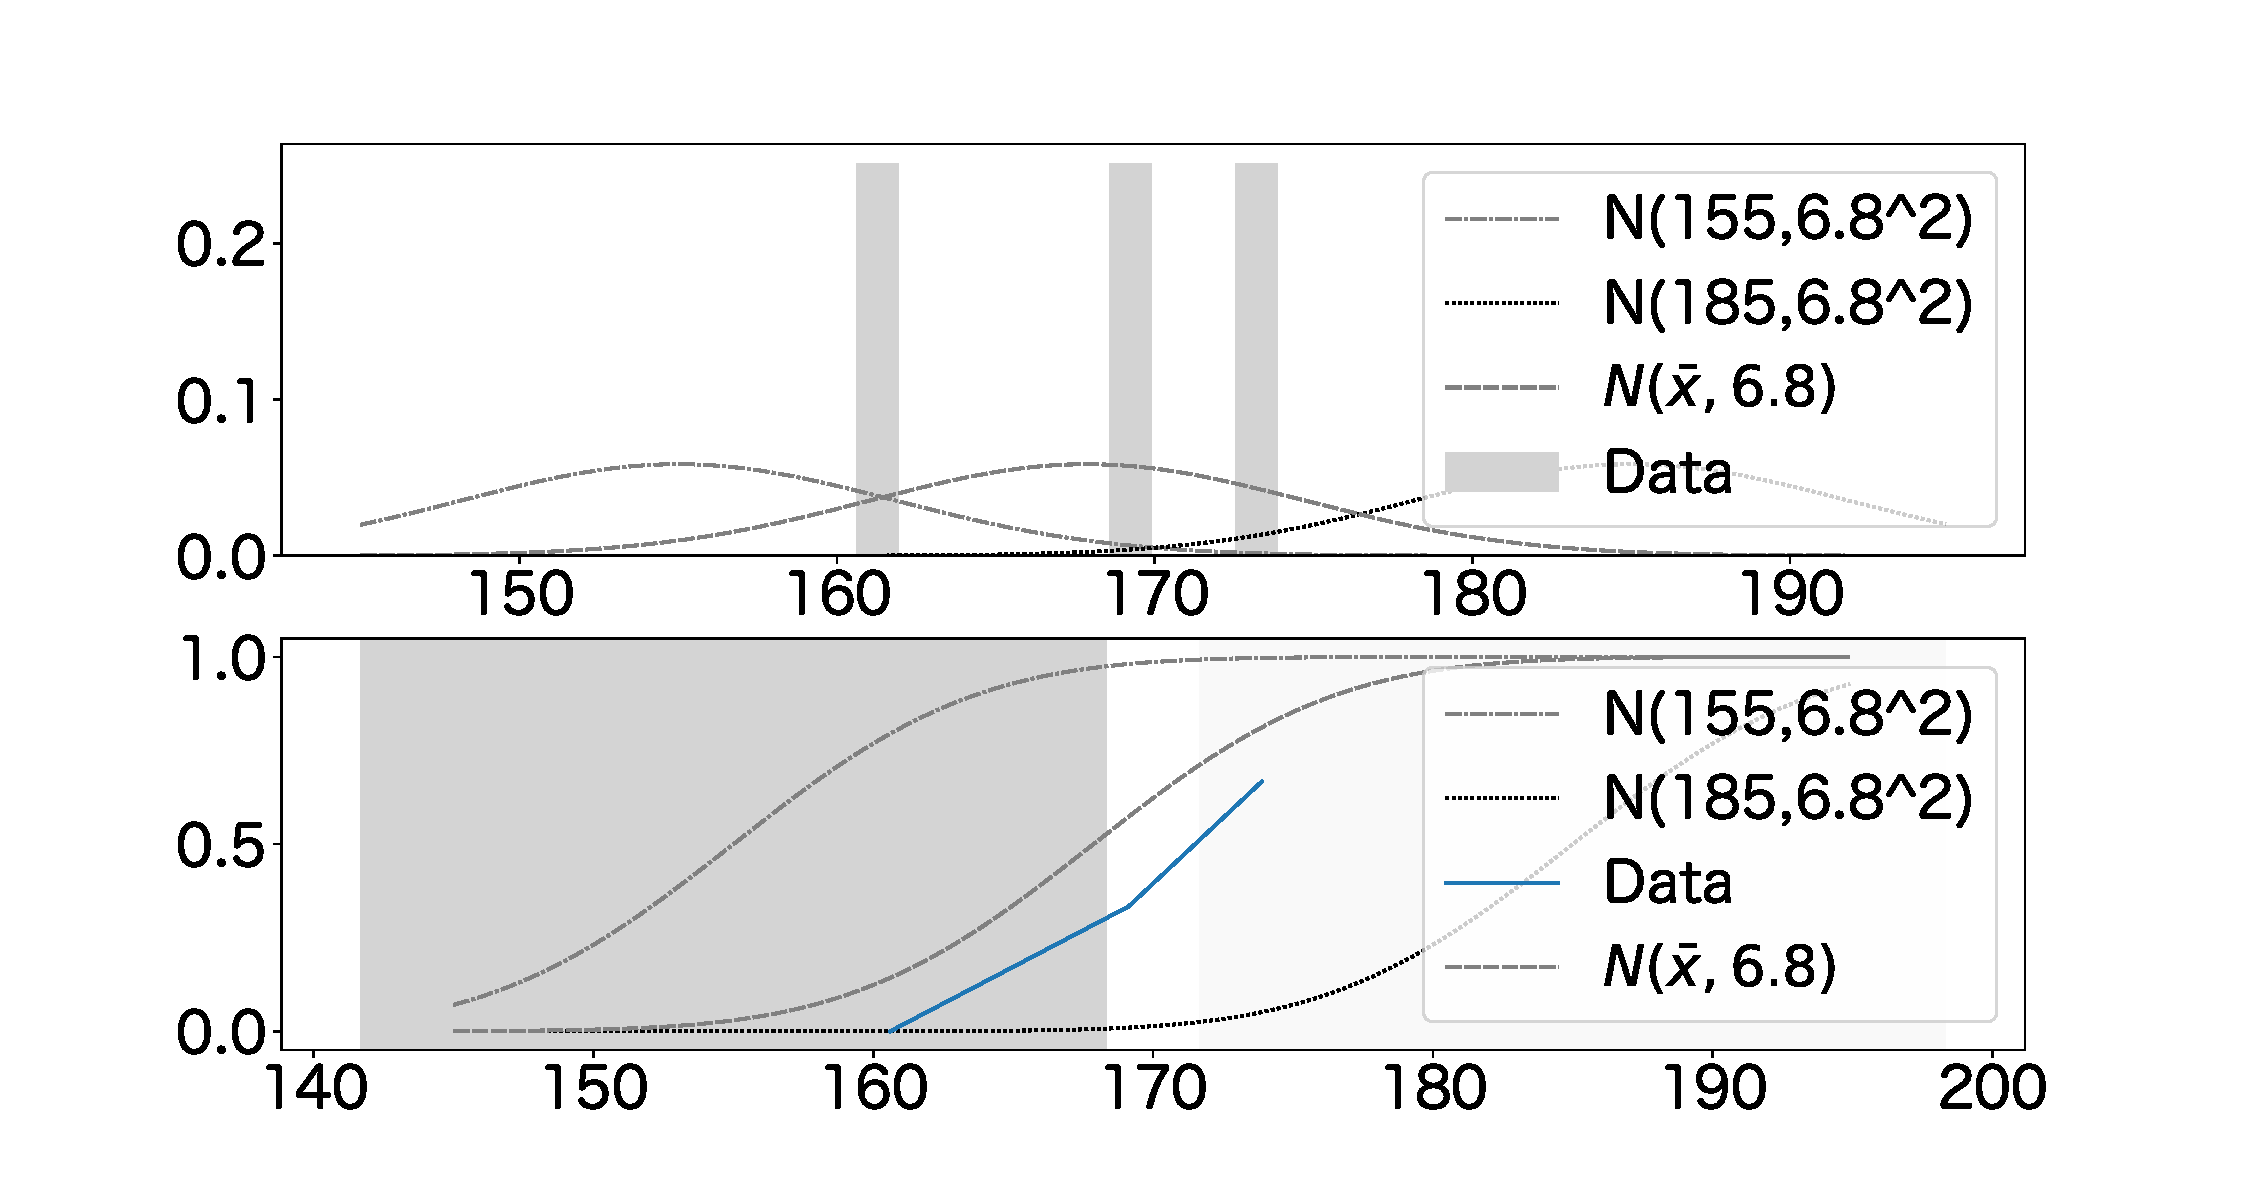
\includegraphics[width=15cm]{./image/02_/maximum_likelihood_false_3.pdf}
        \caption{$N(170,6.8^2)$からサンプルサイズ$3$の標本を得たときの分布。その最尤推定量により求められる分布関数。$N(168,6.8^2),N(171,6.8^2)$の分布関数を示す}
        \label{fig:maximum_likelihood_false_3}
    \end{center}
\end{figure}

\begin{figure}
    \begin{center}
        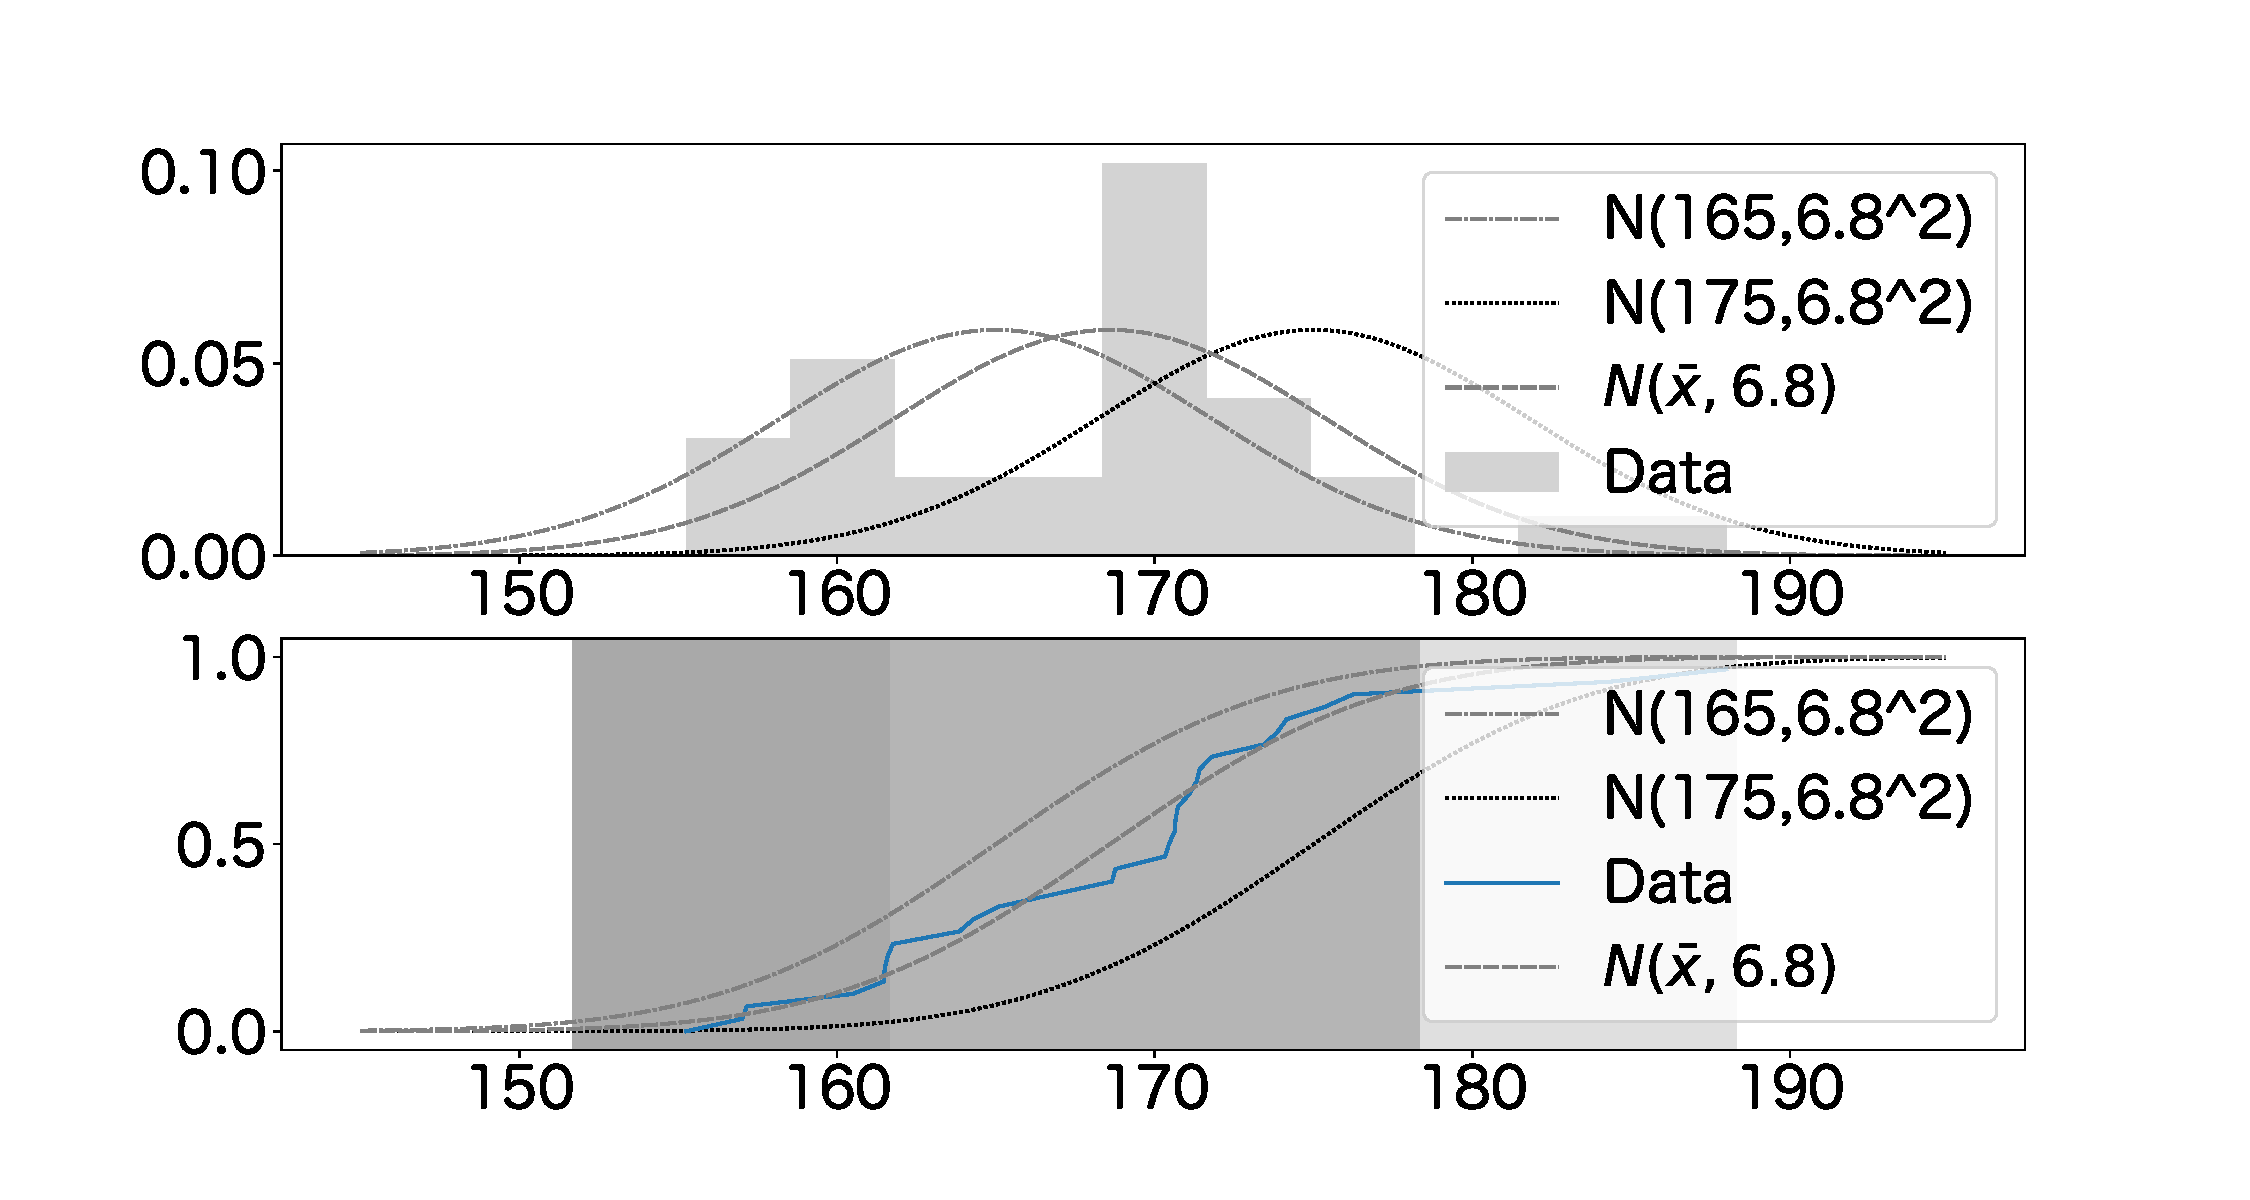
\includegraphics[width=15cm]{./image/02_/maximum_likelihood_false_30.pdf}
        \caption{$N(170,6.8^2)$からサンプルサイズ$3$の標本を得たときの分布。その最尤推定量により求められる分布関数。$N(168,6.8^2),N(171,6.8^2)$の分布関数を示す}
        \label{fig:maximum_likelihood_false_30}
    \end{center}
\end{figure}



\section{標本が統計モデルにより予測可能かを判定する}%統計モデルの性質を使った方法}
%ここまでは、統計モデルの予測がデータと一致することを定量的に評価した。
ここでは、推測に適していないと判断する方法である、統計的仮説検定を紹介する。
この方法は、統計量の一つである統計検定量の統計モデル上での出現しやすさにより、モデルを評価する。


\subsection{モデルの種類}

\begin{table}[hbtp]
    \caption{モデル}
    %\label{table:data_type}
    \centering
    \begin{tabular}{ccc}
      \hline
      モデルの仮定  & 棄却域  &  予測区間 \\
      $M(\mu_0,\sigma_0^2)$ $x_1,x_2,\cdots,x_n\sim N(\mu_0,\sigma_0^2)$  \\
      $\mu_0=\bar{x},\sigma_0^2=\frac{1}{n}\sum(x_i-\bar{x})^2$& -  &  - \\
      $\mu_0,\sigma_0$は設定値とする & $\frac{\sqrt{n}|\bar{x}-\mu_0|}{\sigma_0}\sim N(0,1)$  & $\mu_0-z_{\alpha/2}\frac{\sigma}{\sqrt{n}} <\bar{x}<\mu_0+z_{\alpha/2}\frac{\sigma}{\sqrt{n}}$ \\
      $\mu_0$は設定値,$\sigma^2$は未知 & 
      $|\frac{\bar{x}-\mu_0}{\frac{U}{\sqrt{n}}}| > t_{n-1,\frac{\alpha}{2}}$ただし、$U^2=\frac{1}{n-1}\sum(x_i-\bar{x})$
      %$\mu_0=\bar{x},\sigma_0^2=\frac{1}{n}\sum(x_i-\bar{x})^2$ 
      &  \\
      
      \hline
    \end{tabular}
  \end{table}


\subsection{問題意識}
確率変数$x_1$または、$x_1,x_2,\cdots,x_n$を得たとき、それらが独立同分布に従うという前提のもと、ある母数をもつ分布関数に従う、または従わないと推測することは可能であるだろうか。
最尤推定から、確率変数を得たなら、最尤推定を行って、母数を推測可能な場合がある。
具体的には、正規分布から得られた確率変数については、その平均と分散は、$(\mu,\sigma^2)=(\bar{x},\sum_{i=1}^{n} (x_i-\bar{x})^2/n)$である。

この問題に対して、
正規分布から確率変数を得たとき、ある母数平均$\mu$をもつ正規分布からサンプリングされていないということはできるだろうか。これを議論する。

%\subsection{問題点}
%aa